\documentclass[twoside]{book}

% Packages required by doxygen
\usepackage{calc}
\usepackage{doxygen}
\usepackage{graphicx}
\usepackage[utf8]{inputenc}
\usepackage{makeidx}
\usepackage{multicol}
\usepackage{multirow}
\usepackage{textcomp}
\usepackage[table]{xcolor}

% Font selection
\usepackage[T1]{fontenc}
\usepackage{mathptmx}
\usepackage[scaled=.90]{helvet}
\usepackage{courier}
\usepackage{amssymb}
\usepackage{sectsty}
\renewcommand{\familydefault}{\sfdefault}
\allsectionsfont{%
  \fontseries{bc}\selectfont%
  \color{darkgray}%
}
\renewcommand{\DoxyLabelFont}{%
  \fontseries{bc}\selectfont%
  \color{darkgray}%
}

% Page & text layout
\usepackage{geometry}
\geometry{%
  letterpaper,%
  top=2.5cm,%
  bottom=2.5cm,%
  left=2.5cm,%
  right=2.5cm%
}
\tolerance=750
\hfuzz=15pt
\hbadness=750
\setlength{\emergencystretch}{15pt}
\setlength{\parindent}{0cm}
\setlength{\parskip}{0.2cm}
\makeatletter
\renewcommand{\paragraph}{%
  \@startsection{paragraph}{4}{0ex}{-1.0ex}{1.0ex}{%
    \normalfont\normalsize\bfseries\SS@parafont%
  }%
}
\renewcommand{\subparagraph}{%
  \@startsection{subparagraph}{5}{0ex}{-1.0ex}{1.0ex}{%
    \normalfont\normalsize\bfseries\SS@subparafont%
  }%
}
\makeatother

% Headers & footers
\usepackage{fancyhdr}
\pagestyle{fancyplain}
\fancyhead[LE]{\fancyplain{}{\bfseries\thepage}}
\fancyhead[CE]{\fancyplain{}{}}
\fancyhead[RE]{\fancyplain{}{\bfseries\leftmark}}
\fancyhead[LO]{\fancyplain{}{\bfseries\rightmark}}
\fancyhead[CO]{\fancyplain{}{}}
\fancyhead[RO]{\fancyplain{}{\bfseries\thepage}}
\fancyfoot[LE]{\fancyplain{}{}}
\fancyfoot[CE]{\fancyplain{}{}}
\fancyfoot[RE]{\fancyplain{}{\bfseries\scriptsize Generated on Mon Apr 25 2016 14\-:53\-:27 for Lab 2 Controlling a Motor\-\_\-\-Driver w/ a Task by Doxygen }}
\fancyfoot[LO]{\fancyplain{}{\bfseries\scriptsize Generated on Mon Apr 25 2016 14\-:53\-:27 for Lab 2 Controlling a Motor\-\_\-\-Driver w/ a Task by Doxygen }}
\fancyfoot[CO]{\fancyplain{}{}}
\fancyfoot[RO]{\fancyplain{}{}}
\renewcommand{\footrulewidth}{0.4pt}
\renewcommand{\chaptermark}[1]{%
  \markboth{#1}{}%
}
\renewcommand{\sectionmark}[1]{%
  \markright{\thesection\ #1}%
}

% Indices & bibliography
\usepackage{natbib}
\usepackage[titles]{tocloft}
\setcounter{tocdepth}{3}
\setcounter{secnumdepth}{5}
\makeindex

% Hyperlinks (required, but should be loaded last)
\usepackage{ifpdf}
\ifpdf
  \usepackage[pdftex,pagebackref=true]{hyperref}
\else
  \usepackage[ps2pdf,pagebackref=true]{hyperref}
\fi
\hypersetup{%
  colorlinks=true,%
  linkcolor=blue,%
  citecolor=blue,%
  unicode%
}

% Custom commands
\newcommand{\clearemptydoublepage}{%
  \newpage{\pagestyle{empty}\cleardoublepage}%
}


%===== C O N T E N T S =====

\begin{document}

% Titlepage & ToC
\hypersetup{pageanchor=false}
\pagenumbering{roman}
\begin{titlepage}
\vspace*{7cm}
\begin{center}%
{\Large Lab 2 Controlling a Motor\-\_\-\-Driver w/ a Task \\[1ex]\large v1.\-2 }\\
\vspace*{1cm}
{\large Generated by Doxygen 1.8.6}\\
\vspace*{0.5cm}
{\small Mon Apr 25 2016 14:53:27}\\
\end{center}
\end{titlepage}
\clearemptydoublepage
\tableofcontents
\clearemptydoublepage
\pagenumbering{arabic}
\hypersetup{pageanchor=true}

%--- Begin generated contents ---
\chapter{Hierarchical Index}
\section{Class Hierarchy}
This inheritance list is sorted roughly, but not completely, alphabetically\-:\begin{DoxyCompactList}
\item \contentsline{section}{adc}{\pageref{classadc}}{}
\item \contentsline{section}{motor\-\_\-driver}{\pageref{classmotor__driver}}{}
\item Task\-Base\begin{DoxyCompactList}
\item \contentsline{section}{task\-\_\-brightness}{\pageref{classtask__brightness}}{}
\item \contentsline{section}{task\-\_\-motor}{\pageref{classtask__motor}}{}
\item \contentsline{section}{task\-\_\-user}{\pageref{classtask__user}}{}
\end{DoxyCompactList}
\end{DoxyCompactList}

\chapter{Class Index}
\section{Class List}
Here are the classes, structs, unions and interfaces with brief descriptions:\begin{DoxyCompactList}
\item\contentsline{section}{\hyperlink{classadc}{adc} (This class {\bfseries will} run the A/D converter on an AVR processor )}{\pageref{classadc}}{}
\item\contentsline{section}{\hyperlink{classtask__brightness}{task\_\-brightness} (This task controls the brightness of an LED using an analog input from the A/D converter )}{\pageref{classtask__brightness}}{}
\item\contentsline{section}{\hyperlink{classtask__user}{task\_\-user} }{\pageref{classtask__user}}{}
\end{DoxyCompactList}

\chapter{File Index}
\section{File List}
Here is a list of all documented files with brief descriptions\-:\begin{DoxyCompactList}
\item\contentsline{section}{\hyperlink{adc_8cpp}{adc.\-cpp} }{\pageref{adc_8cpp}}{}
\item\contentsline{section}{\hyperlink{adc_8h}{adc.\-h} }{\pageref{adc_8h}}{}
\item\contentsline{section}{\hyperlink{encoder__driver_8cpp}{encoder\-\_\-driver.\-cpp} \\*This class is the encoder driver class }{\pageref{encoder__driver_8cpp}}{}
\item\contentsline{section}{\hyperlink{encoder__driver_8h}{encoder\-\_\-driver.\-h} \\*This is the header file for the encoder driver class }{\pageref{encoder__driver_8h}}{}
\item\contentsline{section}{\hyperlink{main_8cpp}{main.\-cpp} \\*This is the file for the '\hyperlink{main_8cpp_a840291bc02cba5474a4cb46a9b9566fe}{main()}' function. This function initialzies everything }{\pageref{main_8cpp}}{}
\item\contentsline{section}{\hyperlink{motor__driver_8cpp}{motor\-\_\-driver.\-cpp} \\*This class is the motor driver class }{\pageref{motor__driver_8cpp}}{}
\item\contentsline{section}{\hyperlink{motor__driver_8h}{motor\-\_\-driver.\-h} \\*This is the header file for the '\hyperlink{classmotor__driver}{motor\-\_\-driver}' class }{\pageref{motor__driver_8h}}{}
\item\contentsline{section}{\hyperlink{shares_8h}{shares.\-h} \\*This file contains extern declarations for queues and other inter-\/task data communication objects used in a M\-E405/507/\-Free\-R\-T\-O\-S project }{\pageref{shares_8h}}{}
\item\contentsline{section}{\hyperlink{task__brightness_8cpp}{task\-\_\-brightness.\-cpp} }{\pageref{task__brightness_8cpp}}{}
\item\contentsline{section}{\hyperlink{task__brightness_8h}{task\-\_\-brightness.\-h} }{\pageref{task__brightness_8h}}{}
\item\contentsline{section}{\hyperlink{task__encoder_8cpp}{task\-\_\-encoder.\-cpp} \\*This is the file for the '\hyperlink{classtask__encoder}{task\-\_\-encoder}' class which handles the \hyperlink{classencoder__driver}{encoder\-\_\-driver} class }{\pageref{task__encoder_8cpp}}{}
\item\contentsline{section}{\hyperlink{task__encoder_8h}{task\-\_\-encoder.\-h} \\*This is the header file for the '\hyperlink{classtask__encoder}{task\-\_\-encoder}' class which handles the '\hyperlink{classencoder__driver}{encoder\-\_\-driver}' class }{\pageref{task__encoder_8h}}{}
\item\contentsline{section}{\hyperlink{task__motor_8cpp}{task\-\_\-motor.\-cpp} \\*This class is the task motor class that handles a single motor operation }{\pageref{task__motor_8cpp}}{}
\item\contentsline{section}{\hyperlink{task__motor_8h}{task\-\_\-motor.\-h} \\*This is the header file for the \hyperlink{classtask__motor}{task\-\_\-motor} class }{\pageref{task__motor_8h}}{}
\item\contentsline{section}{\hyperlink{task__user_8cpp}{task\-\_\-user.\-cpp} \\*This is the file for the '\hyperlink{classtask__user}{task\-\_\-user}' class that is what any user will mainly interact with }{\pageref{task__user_8cpp}}{}
\item\contentsline{section}{\hyperlink{task__user_8h}{task\-\_\-user.\-h} \\*This is the header file for the '\hyperlink{classtask__user}{task\-\_\-user}' class }{\pageref{task__user_8h}}{}
\end{DoxyCompactList}

\chapter{Class Documentation}
\hypertarget{classadc}{\section{adc Class Reference}
\label{classadc}\index{adc@{adc}}
}


This class {\bfseries will} run the A/\-D converter on an A\-V\-R processor.  




{\ttfamily \#include $<$adc.\-h$>$}

\subsection*{Public Member Functions}
\begin{DoxyCompactItemize}
\item 
\hyperlink{classadc_af3b8262c08f5fc5ae325a20622883424}{adc} (emstream $\ast$=N\-U\-L\-L)
\begin{DoxyCompactList}\small\item\em This constructor sets up an A/\-D converter. \end{DoxyCompactList}\item 
uint16\-\_\-t \hyperlink{classadc_a2190a59696a7093e1ea605e998ccf97e}{read\-\_\-once} (uint8\-\_\-t)
\begin{DoxyCompactList}\small\item\em This method takes one A/\-D reading from the given channel and returns it. \end{DoxyCompactList}\item 
uint16\-\_\-t \hyperlink{classadc_a58f1030fe64d3dea4ccd8a2687dd6fce}{read\-\_\-oversampled} (uint8\-\_\-t, uint8\-\_\-t)
\begin{DoxyCompactList}\small\item\em This method takes multiple readings specified by an input parameter from a particular channel and return the average of those readings. \end{DoxyCompactList}\end{DoxyCompactItemize}
\subsection*{Protected Attributes}
\begin{DoxyCompactItemize}
\item 
\hypertarget{classadc_a14680b48b723bf1adddd2741ebb18a3e}{emstream $\ast$ \hyperlink{classadc_a14680b48b723bf1adddd2741ebb18a3e}{ptr\-\_\-to\-\_\-serial}}\label{classadc_a14680b48b723bf1adddd2741ebb18a3e}

\begin{DoxyCompactList}\small\item\em The A\-D\-C class uses this pointer to the serial port to say hello. \end{DoxyCompactList}\end{DoxyCompactItemize}


\subsection{Detailed Description}
This class {\bfseries will} run the A/\-D converter on an A\-V\-R processor. 

It has appropriate prototypes for the adc class like methods and constructors in the public region. 

Definition at line 45 of file adc.\-h.



\subsection{Constructor \& Destructor Documentation}
\hypertarget{classadc_af3b8262c08f5fc5ae325a20622883424}{\index{adc@{adc}!adc@{adc}}
\index{adc@{adc}!adc@{adc}}
\subsubsection[{adc}]{\setlength{\rightskip}{0pt plus 5cm}adc\-::adc (
\begin{DoxyParamCaption}
\item[{emstream $\ast$}]{p\-\_\-serial\-\_\-port = {\ttfamily NULL}}
\end{DoxyParamCaption}
)}}\label{classadc_af3b8262c08f5fc5ae325a20622883424}


This constructor sets up an A/\-D converter. 

This constructor takes the pointer given to it and initializes itself. Also, here we set the voltage refrence and enable the A/\-D converter as well as set the prescaler to 32, through some bitshifting. 
\begin{DoxyParams}{Parameters}
{\em p\-\_\-serial\-\_\-port} & A pointer to the serial port which writes debugging info. \\
\hline
\end{DoxyParams}


Definition at line 39 of file adc.\-cpp.



References ptr\-\_\-to\-\_\-serial.



\subsection{Member Function Documentation}
\hypertarget{classadc_a2190a59696a7093e1ea605e998ccf97e}{\index{adc@{adc}!read\-\_\-once@{read\-\_\-once}}
\index{read\-\_\-once@{read\-\_\-once}!adc@{adc}}
\subsubsection[{read\-\_\-once}]{\setlength{\rightskip}{0pt plus 5cm}uint16\-\_\-t adc\-::read\-\_\-once (
\begin{DoxyParamCaption}
\item[{uint8\-\_\-t}]{ch}
\end{DoxyParamCaption}
)}}\label{classadc_a2190a59696a7093e1ea605e998ccf97e}


This method takes one A/\-D reading from the given channel and returns it. 

Given a channel, this method first checks to make sure only valid channels are accepted by setting any outside parameter to channel 0. Then we set the correct register to enable the A/\-D and use a while loop to wait until the completion bit is 0. At that point, the loop breaks and the results stored in A\-D\-C\-L and A\-D\-C\-H are concatenated into the 16 bit return value. 
\begin{DoxyParams}{Parameters}
{\em ch} & The A/\-D channel which is being read must be from 0 to 7 \\
\hline
\end{DoxyParams}
\begin{DoxyReturn}{Returns}
A\-D\-C\-\_\-value, the 16 bit returned value of the concatendated High and Low results. 
\end{DoxyReturn}


Definition at line 66 of file adc.\-cpp.



Referenced by read\-\_\-oversampled().

\hypertarget{classadc_a58f1030fe64d3dea4ccd8a2687dd6fce}{\index{adc@{adc}!read\-\_\-oversampled@{read\-\_\-oversampled}}
\index{read\-\_\-oversampled@{read\-\_\-oversampled}!adc@{adc}}
\subsubsection[{read\-\_\-oversampled}]{\setlength{\rightskip}{0pt plus 5cm}uint16\-\_\-t adc\-::read\-\_\-oversampled (
\begin{DoxyParamCaption}
\item[{uint8\-\_\-t}]{channel, }
\item[{uint8\-\_\-t}]{samples}
\end{DoxyParamCaption}
)}}\label{classadc_a58f1030fe64d3dea4ccd8a2687dd6fce}


This method takes multiple readings specified by an input parameter from a particular channel and return the average of those readings. 


\begin{DoxyParams}{Parameters}
{\em channel} & this parameter specifies which channel we're going to be averaging \\
\hline
{\em samples} & this specifies how many samples we're going to be taking and serves as the basis for our average division. \\
\hline
\end{DoxyParams}
\begin{DoxyReturn}{Returns}
average\-\_\-result, this is the average value read over that channel per those samples. 
\end{DoxyReturn}


Definition at line 101 of file adc.\-cpp.



References read\-\_\-once().



The documentation for this class was generated from the following files\-:\begin{DoxyCompactItemize}
\item 
\hyperlink{adc_8h}{adc.\-h}\item 
\hyperlink{adc_8cpp}{adc.\-cpp}\end{DoxyCompactItemize}

\hypertarget{classmotor__driver}{\section{motor\-\_\-driver Class Reference}
\label{classmotor__driver}\index{motor\-\_\-driver@{motor\-\_\-driver}}
}


This class will run the D\-C motor.  




{\ttfamily \#include $<$motor\-\_\-driver.\-h$>$}

\subsection*{Public Member Functions}
\begin{DoxyCompactItemize}
\item 
\hyperlink{classmotor__driver_a2c184d7e66a7935c0347d72b44d37c62}{motor\-\_\-driver} (emstream $\ast$serial\-\_\-\-P\-O\-R\-T\-\_\-incoming, volatile uint8\-\_\-t $\ast$input\-\_\-\-P\-O\-R\-T\-\_\-incoming, volatile uint8\-\_\-t $\ast$diag\-\_\-\-P\-O\-R\-T\-\_\-incoming, volatile uint8\-\_\-t $\ast$pwm\-\_\-\-P\-O\-R\-T\-\_\-incoming, volatile uint16\-\_\-t $\ast$ocr\-\_\-\-P\-O\-R\-T\-\_\-incoming, uint8\-\_\-t input\-\_\-\-A\-P\-I\-N\-\_\-incoming, uint8\-\_\-t input\-\_\-\-B\-P\-I\-N\-\_\-incoming, uint8\-\_\-t diag\-\_\-\-P\-I\-N\-\_\-incoming, uint8\-\_\-t pwm\-\_\-\-P\-I\-N\-\_\-incoming)
\begin{DoxyCompactList}\small\item\em set the public constructor and the public methods \end{DoxyCompactList}\item 
void \hyperlink{classmotor__driver_a2bc43c500da3297a815c5958bee57f20}{set\-\_\-power} (int16\-\_\-t)
\begin{DoxyCompactList}\small\item\em prototype for set\-\_\-power method of \hyperlink{classmotor__driver}{motor\-\_\-driver} \end{DoxyCompactList}\item 
void \hyperlink{classmotor__driver_a0ceae2119e7bc1a03f409ca9c0cce32c}{brake} (int16\-\_\-t)
\begin{DoxyCompactList}\small\item\em prototype for the brake method of \hyperlink{classmotor__driver}{motor\-\_\-driver} with parameter \end{DoxyCompactList}\item 
void \hyperlink{classmotor__driver_aa21e7894053cd83968d9e6b2958c9aec}{brake} (void)
\begin{DoxyCompactList}\small\item\em prototype for brake method w/o parameter \end{DoxyCompactList}\end{DoxyCompactItemize}
\subsection*{Public Attributes}
\begin{DoxyCompactItemize}
\item 
\hypertarget{classmotor__driver_a960f4685dd5db6cbbe29399dbaf1a8f7}{volatile uint16\-\_\-t $\ast$ \hyperlink{classmotor__driver_a960f4685dd5db6cbbe29399dbaf1a8f7}{ocr\-\_\-\-P\-O\-R\-T}}\label{classmotor__driver_a960f4685dd5db6cbbe29399dbaf1a8f7}

\begin{DoxyCompactList}\small\item\em pointer to the comp register \end{DoxyCompactList}\end{DoxyCompactItemize}
\subsection*{Protected Attributes}
\begin{DoxyCompactItemize}
\item 
\hypertarget{classmotor__driver_a98a0c18a3b4d8b61266f98437aab12a9}{emstream $\ast$ \hyperlink{classmotor__driver_a98a0c18a3b4d8b61266f98437aab12a9}{serial\-\_\-\-P\-O\-R\-T}}\label{classmotor__driver_a98a0c18a3b4d8b61266f98437aab12a9}

\begin{DoxyCompactList}\small\item\em The \hyperlink{classmotor__driver}{motor\-\_\-driver} class uses this pointer to the serial port to say hello. \end{DoxyCompactList}\item 
\hypertarget{classmotor__driver_aa9ce032000d0eb28499df3fa53255022}{volatile uint8\-\_\-t $\ast$ \hyperlink{classmotor__driver_aa9ce032000d0eb28499df3fa53255022}{input\-\_\-\-D\-D\-R}}\label{classmotor__driver_aa9ce032000d0eb28499df3fa53255022}

\begin{DoxyCompactList}\small\item\em pointer to input D\-D\-R register \end{DoxyCompactList}\item 
\hypertarget{classmotor__driver_ad821a9c32c2e296373f5273db99e3f59}{volatile uint8\-\_\-t $\ast$ \hyperlink{classmotor__driver_ad821a9c32c2e296373f5273db99e3f59}{input\-\_\-\-P\-O\-R\-T}}\label{classmotor__driver_ad821a9c32c2e296373f5273db99e3f59}

\begin{DoxyCompactList}\small\item\em pointer to the data input register \end{DoxyCompactList}\item 
\hypertarget{classmotor__driver_a6b1aa2bcd4eecada6abe2e3d11fecd88}{volatile uint8\-\_\-t $\ast$ \hyperlink{classmotor__driver_a6b1aa2bcd4eecada6abe2e3d11fecd88}{diag\-\_\-\-D\-D\-R}}\label{classmotor__driver_a6b1aa2bcd4eecada6abe2e3d11fecd88}

\begin{DoxyCompactList}\small\item\em pointer to diagnostic register \end{DoxyCompactList}\item 
\hypertarget{classmotor__driver_af0259585bf3d8d7a3cf236913255a543}{volatile uint8\-\_\-t $\ast$ \hyperlink{classmotor__driver_af0259585bf3d8d7a3cf236913255a543}{diag\-\_\-\-P\-O\-R\-T}}\label{classmotor__driver_af0259585bf3d8d7a3cf236913255a543}

\begin{DoxyCompactList}\small\item\em pointer to the diag input register \end{DoxyCompactList}\item 
\hypertarget{classmotor__driver_a1828fd490bb9fa20d9a1974db7bea08a}{volatile uint8\-\_\-t $\ast$ \hyperlink{classmotor__driver_a1828fd490bb9fa20d9a1974db7bea08a}{pwm\-\_\-\-D\-D\-R}}\label{classmotor__driver_a1828fd490bb9fa20d9a1974db7bea08a}

\begin{DoxyCompactList}\small\item\em pointer to D\-D\-R pwm register \end{DoxyCompactList}\item 
\hypertarget{classmotor__driver_ad7108a5cc11ba229ed117cb6c98adda6}{volatile uint8\-\_\-t $\ast$ \hyperlink{classmotor__driver_ad7108a5cc11ba229ed117cb6c98adda6}{pwm\-\_\-\-P\-O\-R\-T}}\label{classmotor__driver_ad7108a5cc11ba229ed117cb6c98adda6}

\begin{DoxyCompactList}\small\item\em pointer to pwm port \end{DoxyCompactList}\item 
\hypertarget{classmotor__driver_a0f3eeec4986d707cfcd5d25a6dd5fac9}{uint8\-\_\-t \hyperlink{classmotor__driver_a0f3eeec4986d707cfcd5d25a6dd5fac9}{input\-\_\-\-A\-P\-I\-N}}\label{classmotor__driver_a0f3eeec4986d707cfcd5d25a6dd5fac9}

\begin{DoxyCompactList}\small\item\em pin\-A value to set the input register \end{DoxyCompactList}\item 
\hypertarget{classmotor__driver_a079434aa37c0edbdbce3c1c04ffc0e0a}{uint8\-\_\-t \hyperlink{classmotor__driver_a079434aa37c0edbdbce3c1c04ffc0e0a}{input\-\_\-\-B\-P\-I\-N}}\label{classmotor__driver_a079434aa37c0edbdbce3c1c04ffc0e0a}

\begin{DoxyCompactList}\small\item\em pin\-B value to set the input register \end{DoxyCompactList}\item 
\hypertarget{classmotor__driver_ad97987799de2b9467ce7b01f5b291fcb}{uint8\-\_\-t \hyperlink{classmotor__driver_ad97987799de2b9467ce7b01f5b291fcb}{diag\-\_\-\-P\-I\-N}}\label{classmotor__driver_ad97987799de2b9467ce7b01f5b291fcb}

\begin{DoxyCompactList}\small\item\em pin valye to set the diag register \end{DoxyCompactList}\item 
\hypertarget{classmotor__driver_accfb1e4405787b56c89636f5a14b5762}{uint8\-\_\-t \hyperlink{classmotor__driver_accfb1e4405787b56c89636f5a14b5762}{pwm\-\_\-\-P\-I\-N}}\label{classmotor__driver_accfb1e4405787b56c89636f5a14b5762}

\begin{DoxyCompactList}\small\item\em pin value to set the pwm register \end{DoxyCompactList}\end{DoxyCompactItemize}


\subsection{Detailed Description}
This class will run the D\-C motor. 

This class sets up a driver for a D\-C motor to be used with the H bridge on the custom Atmega1281 board. It sets up no private variables, and has multiple protected variables. The protected variables include 6 pointers to registers that hold the correct data for the 

Definition at line 62 of file motor\-\_\-driver.\-h.



\subsection{Constructor \& Destructor Documentation}
\hypertarget{classmotor__driver_a2c184d7e66a7935c0347d72b44d37c62}{\index{motor\-\_\-driver@{motor\-\_\-driver}!motor\-\_\-driver@{motor\-\_\-driver}}
\index{motor\-\_\-driver@{motor\-\_\-driver}!motor_driver@{motor\-\_\-driver}}
\subsubsection[{motor\-\_\-driver}]{\setlength{\rightskip}{0pt plus 5cm}motor\-\_\-driver\-::motor\-\_\-driver (
\begin{DoxyParamCaption}
\item[{emstream $\ast$}]{serial\-\_\-\-P\-O\-R\-T\-\_\-incoming, }
\item[{volatile uint8\-\_\-t $\ast$}]{input\-\_\-\-P\-O\-R\-T\-\_\-incoming, }
\item[{volatile uint8\-\_\-t $\ast$}]{diag\-\_\-\-P\-O\-R\-T\-\_\-incoming, }
\item[{volatile uint8\-\_\-t $\ast$}]{pwm\-\_\-\-P\-O\-R\-T\-\_\-incoming, }
\item[{volatile uint16\-\_\-t $\ast$}]{ocr\-\_\-\-P\-O\-R\-T\-\_\-incoming, }
\item[{uint8\-\_\-t}]{input\-\_\-\-A\-P\-I\-N\-\_\-incoming, }
\item[{uint8\-\_\-t}]{input\-\_\-\-B\-P\-I\-N\-\_\-incoming, }
\item[{uint8\-\_\-t}]{diag\-\_\-\-P\-I\-N\-\_\-incoming, }
\item[{uint8\-\_\-t}]{pwm\-\_\-\-P\-I\-N\-\_\-incoming}
\end{DoxyParamCaption}
)}}\label{classmotor__driver_a2c184d7e66a7935c0347d72b44d37c62}


set the public constructor and the public methods 

This is the constuctor for the \hyperlink{classmotor__driver}{motor\-\_\-driver} class.

This constructor takes in several addresses and delivers them to the protected variables declared in our header file.


\begin{DoxyParams}[1]{Parameters}
 & {\em serial\-\_\-\-P\-O\-R\-T\-\_\-incoming} & This holds the address to the incoming data register \\
\hline
 & {\em input\-\_\-\-P\-O\-R\-T\-\_\-incoming} & This holds the address to the incoming data register \\
\hline
 & {\em diag\-\_\-\-P\-O\-R\-T\-\_\-incoming} & This holds address port to incoming diag port reg \\
\hline
 & {\em pwm\-\_\-\-P\-O\-R\-T\-\_\-incoming} & This holds the address to the incoming data register \\
\hline
 & {\em ocr\-\_\-\-P\-O\-R\-T\-\_\-incoming} & This holds the address to the incoming ocr register \\
\hline
\mbox{\tt in}  & {\em input\-\_\-\-A\-P\-I\-N\-\_\-incoming} & This holds defined value for I\-N\-A pin \\
\hline
\mbox{\tt in}  & {\em input\-\_\-\-B\-P\-I\-N\-\_\-incoming} & This holds defined value for I\-N\-B pin \\
\hline
\mbox{\tt in}  & {\em diag\-\_\-\-P\-I\-N\-\_\-incoming} & This holds defined value for appropriate diag ping \\
\hline
\mbox{\tt in}  & {\em pwm\-\_\-\-P\-I\-N\-\_\-incoming} & This holds defined value for pwm pin \\
\hline
\end{DoxyParams}


Definition at line 69 of file motor\-\_\-driver.\-cpp.



References diag\-\_\-\-D\-D\-R, diag\-\_\-\-P\-I\-N, diag\-\_\-\-P\-O\-R\-T, input\-\_\-\-A\-P\-I\-N, input\-\_\-\-B\-P\-I\-N, input\-\_\-\-D\-D\-R, input\-\_\-\-P\-O\-R\-T, ocr\-\_\-\-P\-O\-R\-T, pwm\-\_\-\-D\-D\-R, pwm\-\_\-\-P\-I\-N, pwm\-\_\-\-P\-O\-R\-T, and serial\-\_\-\-P\-O\-R\-T.



\subsection{Member Function Documentation}
\hypertarget{classmotor__driver_a0ceae2119e7bc1a03f409ca9c0cce32c}{\index{motor\-\_\-driver@{motor\-\_\-driver}!brake@{brake}}
\index{brake@{brake}!motor_driver@{motor\-\_\-driver}}
\subsubsection[{brake}]{\setlength{\rightskip}{0pt plus 5cm}void motor\-\_\-driver\-::brake (
\begin{DoxyParamCaption}
\item[{int16\-\_\-t}]{f\-\_\-brake}
\end{DoxyParamCaption}
)}}\label{classmotor__driver_a0ceae2119e7bc1a03f409ca9c0cce32c}


prototype for the brake method of \hyperlink{classmotor__driver}{motor\-\_\-driver} with parameter 

This method actively brakes by setting both pins high. This is stronger braking than just letting it freewheel.


\begin{DoxyParams}[1]{Parameters}
\mbox{\tt in}  & {\em f\-\_\-brake} & The f brake is a signal that will indicate brake power \\
\hline
\end{DoxyParams}


Definition at line 216 of file motor\-\_\-driver.\-cpp.



References diag\-\_\-\-D\-D\-R, diag\-\_\-\-P\-I\-N, diag\-\_\-\-P\-O\-R\-T, input\-\_\-\-A\-P\-I\-N, input\-\_\-\-B\-P\-I\-N, input\-\_\-\-D\-D\-R, input\-\_\-\-P\-O\-R\-T, pwm\-\_\-\-D\-D\-R, and pwm\-\_\-\-P\-I\-N.

\hypertarget{classmotor__driver_aa21e7894053cd83968d9e6b2958c9aec}{\index{motor\-\_\-driver@{motor\-\_\-driver}!brake@{brake}}
\index{brake@{brake}!motor_driver@{motor\-\_\-driver}}
\subsubsection[{brake}]{\setlength{\rightskip}{0pt plus 5cm}void motor\-\_\-driver\-::brake (
\begin{DoxyParamCaption}
\item[{void}]{}
\end{DoxyParamCaption}
)}}\label{classmotor__driver_aa21e7894053cd83968d9e6b2958c9aec}


prototype for brake method w/o parameter 

This method sets both H Drive pins low to let the motor freewheel. 

Definition at line 249 of file motor\-\_\-driver.\-cpp.



References diag\-\_\-\-D\-D\-R, diag\-\_\-\-P\-I\-N, diag\-\_\-\-P\-O\-R\-T, input\-\_\-\-A\-P\-I\-N, input\-\_\-\-B\-P\-I\-N, input\-\_\-\-D\-D\-R, input\-\_\-\-P\-O\-R\-T, pwm\-\_\-\-D\-D\-R, and pwm\-\_\-\-P\-I\-N.

\hypertarget{classmotor__driver_a2bc43c500da3297a815c5958bee57f20}{\index{motor\-\_\-driver@{motor\-\_\-driver}!set\-\_\-power@{set\-\_\-power}}
\index{set\-\_\-power@{set\-\_\-power}!motor_driver@{motor\-\_\-driver}}
\subsubsection[{set\-\_\-power}]{\setlength{\rightskip}{0pt plus 5cm}void motor\-\_\-driver\-::set\-\_\-power (
\begin{DoxyParamCaption}
\item[{int16\-\_\-t}]{sig}
\end{DoxyParamCaption}
)}}\label{classmotor__driver_a2bc43c500da3297a815c5958bee57f20}


prototype for set\-\_\-power method of \hyperlink{classmotor__driver}{motor\-\_\-driver} 

This method sets the appropriate input direction based on the incoming pwm parameter labeled power.


\begin{DoxyParams}[1]{Parameters}
\mbox{\tt in}  & {\em sig} & the incoming signed input that tells our pwm signal going into the Output/\-Compare how strong the motor will be moving \\
\hline
\end{DoxyParams}


Definition at line 143 of file motor\-\_\-driver.\-cpp.



References diag\-\_\-\-D\-D\-R, diag\-\_\-\-P\-I\-N, diag\-\_\-\-P\-O\-R\-T, input\-\_\-\-A\-P\-I\-N, input\-\_\-\-B\-P\-I\-N, input\-\_\-\-D\-D\-R, input\-\_\-\-P\-O\-R\-T, ocr\-\_\-\-P\-O\-R\-T, pwm\-\_\-\-D\-D\-R, and pwm\-\_\-\-P\-I\-N.



Referenced by task\-\_\-motor\-::run().



The documentation for this class was generated from the following files\-:\begin{DoxyCompactItemize}
\item 
\hyperlink{motor__driver_8h}{motor\-\_\-driver.\-h}\item 
\hyperlink{motor__driver_8cpp}{motor\-\_\-driver.\-cpp}\end{DoxyCompactItemize}

\hypertarget{classtask__brightness}{\section{task\-\_\-brightness Class Reference}
\label{classtask__brightness}\index{task\-\_\-brightness@{task\-\_\-brightness}}
}


This task controls the brightness of an L\-E\-D based on input from an A/\-D converter that also drives 2 motors.  




{\ttfamily \#include $<$task\-\_\-brightness.\-h$>$}

Inheritance diagram for task\-\_\-brightness\-:\begin{figure}[H]
\begin{center}
\leavevmode
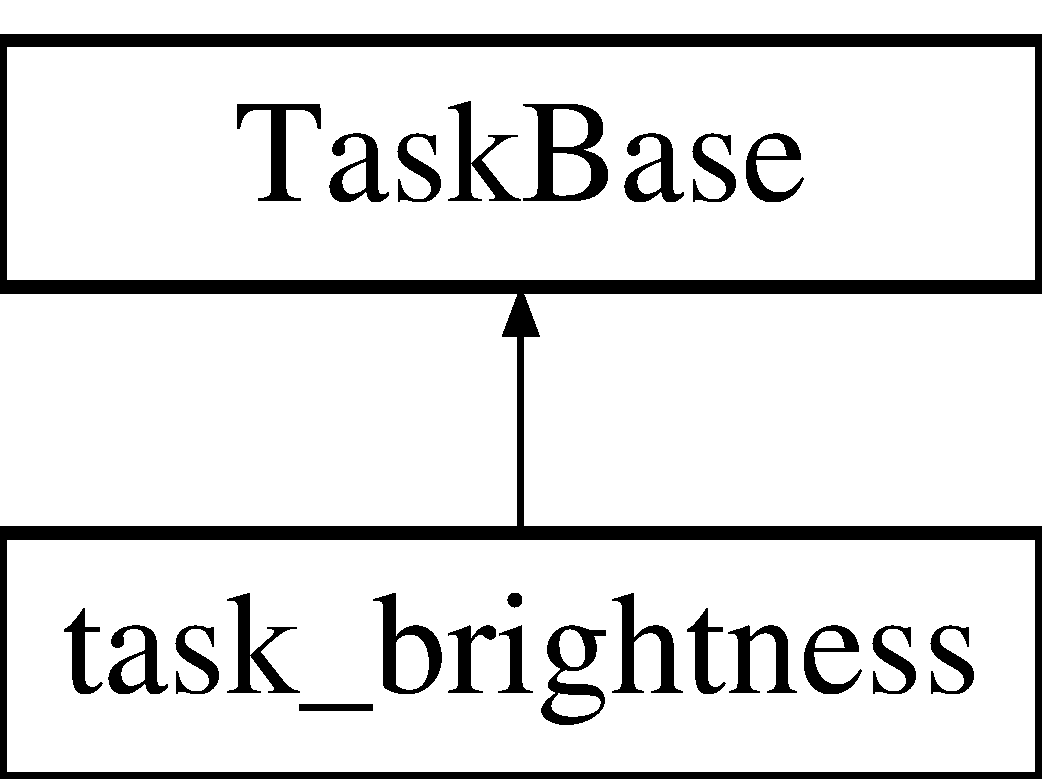
\includegraphics[height=2.000000cm]{classtask__brightness}
\end{center}
\end{figure}
\subsection*{Public Member Functions}
\begin{DoxyCompactItemize}
\item 
\hyperlink{classtask__brightness_a5802baf3a0c9fe53ccbce8966d1fad47}{task\-\_\-brightness} (const char $\ast$, unsigned port\-B\-A\-S\-E\-\_\-\-T\-Y\-P\-E, size\-\_\-t, emstream $\ast$)
\item 
void \hyperlink{classtask__brightness_a615beac07a99f0856f048a46fd9a3898}{run} (void)
\end{DoxyCompactItemize}


\subsection{Detailed Description}
This task controls the brightness of an L\-E\-D based on input from an A/\-D converter that also drives 2 motors. 

The A/\-D converter is run using a driver in files {\ttfamily \hyperlink{adc_8h}{adc.\-h}} and {\ttfamily \hyperlink{adc_8cpp}{adc.\-cpp}}. and the \hyperlink{classmotor__driver}{motor\-\_\-driver} is run using a driver in files {\ttfamily \hyperlink{motor__driver_8h}{motor\-\_\-driver.\-h}} and {\ttfamily \hyperlink{motor__driver_8cpp}{motor\-\_\-driver.\-cpp}} Code in this task sets up a timer/counter in P\-W\-M mode and controls the L\-E\-D's average brightness through Timer/\-Counter 3 and the Timer/\-Counter 1 in fast non-\/inverted P\-W\-M sets up the correct input for the pwm of the motor. 

Definition at line 59 of file task\-\_\-brightness.\-h.



\subsection{Constructor \& Destructor Documentation}
\hypertarget{classtask__brightness_a5802baf3a0c9fe53ccbce8966d1fad47}{\index{task\-\_\-brightness@{task\-\_\-brightness}!task\-\_\-brightness@{task\-\_\-brightness}}
\index{task\-\_\-brightness@{task\-\_\-brightness}!task_brightness@{task\-\_\-brightness}}
\subsubsection[{task\-\_\-brightness}]{\setlength{\rightskip}{0pt plus 5cm}task\-\_\-brightness\-::task\-\_\-brightness (
\begin{DoxyParamCaption}
\item[{const char $\ast$}]{a\-\_\-name, }
\item[{unsigned port\-B\-A\-S\-E\-\_\-\-T\-Y\-P\-E}]{a\-\_\-priority, }
\item[{size\-\_\-t}]{a\-\_\-stack\-\_\-size, }
\item[{emstream $\ast$}]{p\-\_\-ser\-\_\-dev}
\end{DoxyParamCaption}
)}}\label{classtask__brightness_a5802baf3a0c9fe53ccbce8966d1fad47}
This constructor creates a task which controls the brightness of an L\-E\-D using input from an A/\-D converter. The main job of this constructor is to call the constructor of parent class ({\ttfamily frt\-\_\-task} ); the parent's constructor the work. 
\begin{DoxyParams}{Parameters}
{\em a\-\_\-name} & A character string which will be the name of this task \\
\hline
{\em a\-\_\-priority} & The priority at which this task will initially run (default\-: 0) \\
\hline
{\em a\-\_\-stack\-\_\-size} & The size of this task's stack in bytes (default\-: config\-M\-I\-N\-I\-M\-A\-L\-\_\-\-S\-T\-A\-C\-K\-\_\-\-S\-I\-Z\-E) \\
\hline
{\em p\-\_\-ser\-\_\-dev} & Pointer to a serial device (port, radio, S\-D card, etc.) which can be used by this task to communicate (default\-: N\-U\-L\-L) \\
\hline
\end{DoxyParams}


Definition at line 49 of file task\-\_\-brightness.\-cpp.



\subsection{Member Function Documentation}
\hypertarget{classtask__brightness_a615beac07a99f0856f048a46fd9a3898}{\index{task\-\_\-brightness@{task\-\_\-brightness}!run@{run}}
\index{run@{run}!task_brightness@{task\-\_\-brightness}}
\subsubsection[{run}]{\setlength{\rightskip}{0pt plus 5cm}void task\-\_\-brightness\-::run (
\begin{DoxyParamCaption}
\item[{void}]{}
\end{DoxyParamCaption}
)}}\label{classtask__brightness_a615beac07a99f0856f048a46fd9a3898}
@ brief This method is called once by the R\-T\-O\-S scheduler. @ details Each time around the for (;;) loop, it reads the A/\-D converter and uses the result to control the brightness of an L\-E\-D. It also uses the input from the adc object to control the speed and direction of any motor driver object declared. 

Definition at line 67 of file task\-\_\-brightness.\-cpp.



The documentation for this class was generated from the following files\-:\begin{DoxyCompactItemize}
\item 
\hyperlink{task__brightness_8h}{task\-\_\-brightness.\-h}\item 
\hyperlink{task__brightness_8cpp}{task\-\_\-brightness.\-cpp}\end{DoxyCompactItemize}

\hypertarget{classtask__motor}{\section{task\-\_\-motor Class Reference}
\label{classtask__motor}\index{task\-\_\-motor@{task\-\_\-motor}}
}


This class is the task motor class that handles a single motor operation.  




{\ttfamily \#include $<$task\-\_\-motor.\-h$>$}

Inheritance diagram for task\-\_\-motor\-:\begin{figure}[H]
\begin{center}
\leavevmode
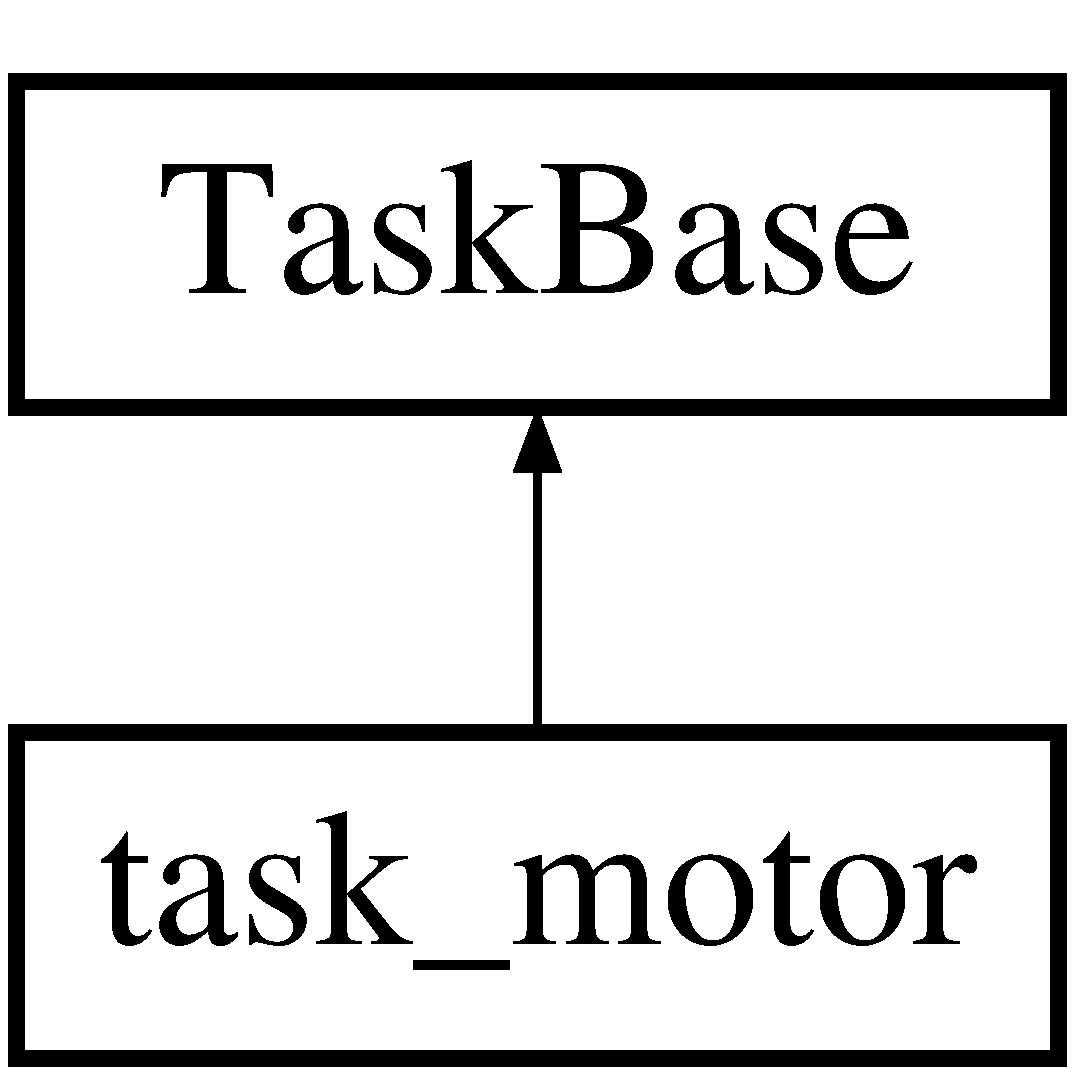
\includegraphics[height=2.000000cm]{classtask__motor}
\end{center}
\end{figure}
\subsection*{Public Member Functions}
\begin{DoxyCompactItemize}
\item 
\hyperlink{classtask__motor_aefd82ba00ba8755bad9fdb516719b3d5}{task\-\_\-motor} (const char $\ast$, unsigned port\-B\-A\-S\-E\-\_\-\-T\-Y\-P\-E, size\-\_\-t, emstream $\ast$, \hyperlink{classmotor__driver}{motor\-\_\-driver} $\ast$, \hyperlink{classadc}{adc} $\ast$, uint8\-\_\-t)
\begin{DoxyCompactList}\small\item\em This constructor creates a generic task of which many copies can be made. \end{DoxyCompactList}\item 
void \hyperlink{classtask__motor_a895a075ec470c9d5a07b8959de06aacd}{run} (void)
\begin{DoxyCompactList}\small\item\em This method is called by the R\-T\-O\-S once to run the task loop for ever and ever. \end{DoxyCompactList}\end{DoxyCompactItemize}
\subsection*{Protected Attributes}
\begin{DoxyCompactItemize}
\item 
uint8\-\_\-t \hyperlink{classtask__motor_aeb4767ff390d9f8bd9f37dfcab0daa4b}{motor\-\_\-identifier}
\begin{DoxyCompactList}\small\item\em No private variables or methods for this class. \end{DoxyCompactList}\item 
\hypertarget{classtask__motor_aa2ed8c7d16f05cb57b11e86bdc7e646b}{\hyperlink{classmotor__driver}{motor\-\_\-driver} $\ast$ \hyperlink{classtask__motor_aa2ed8c7d16f05cb57b11e86bdc7e646b}{motor}}\label{classtask__motor_aa2ed8c7d16f05cb57b11e86bdc7e646b}

\begin{DoxyCompactList}\small\item\em This holds the pointer to the motor that this task will control. \end{DoxyCompactList}\item 
\hypertarget{classtask__motor_a388438912d463a7cb919dc6dbdcb2353}{\hyperlink{classadc}{adc} $\ast$ \hyperlink{classtask__motor_a388438912d463a7cb919dc6dbdcb2353}{p\-\_\-adc}}\label{classtask__motor_a388438912d463a7cb919dc6dbdcb2353}

\begin{DoxyCompactList}\small\item\em variable pointer that points to the A/\-D Converter given by \hyperlink{main_8cpp_a840291bc02cba5474a4cb46a9b9566fe}{main()} \end{DoxyCompactList}\end{DoxyCompactItemize}


\subsection{Detailed Description}
This class is the task motor class that handles a single motor operation. 

This is a task class that will control the operation of its own motor driver given to it as a pointer and initiated in the \hyperlink{main_8cpp_a840291bc02cba5474a4cb46a9b9566fe}{main()} function. it lays out the logic necessary to make commands from \hyperlink{classtask__user}{task\-\_\-user} to the motor driver happen. 

Definition at line 72 of file task\-\_\-motor.\-h.



\subsection{Constructor \& Destructor Documentation}
\hypertarget{classtask__motor_aefd82ba00ba8755bad9fdb516719b3d5}{\index{task\-\_\-motor@{task\-\_\-motor}!task\-\_\-motor@{task\-\_\-motor}}
\index{task\-\_\-motor@{task\-\_\-motor}!task_motor@{task\-\_\-motor}}
\subsubsection[{task\-\_\-motor}]{\setlength{\rightskip}{0pt plus 5cm}task\-\_\-motor\-::task\-\_\-motor (
\begin{DoxyParamCaption}
\item[{const char $\ast$}]{a\-\_\-name, }
\item[{unsigned port\-B\-A\-S\-E\-\_\-\-T\-Y\-P\-E}]{a\-\_\-priority, }
\item[{size\-\_\-t}]{a\-\_\-stack\-\_\-size, }
\item[{emstream $\ast$}]{p\-\_\-ser\-\_\-dev, }
\item[{{\bf motor\-\_\-driver} $\ast$}]{motor\-\_\-inc, }
\item[{{\bf adc} $\ast$}]{adc\-\_\-inc, }
\item[{uint8\-\_\-t}]{motor\-\_\-id\-\_\-inc}
\end{DoxyParamCaption}
)}}\label{classtask__motor_aefd82ba00ba8755bad9fdb516719b3d5}


This constructor creates a generic task of which many copies can be made. 

This constructor builds an instance of a \hyperlink{classtask__motor}{task\-\_\-motor} that will be used to control a motor unique to the task.


\begin{DoxyParams}[1]{Parameters}
\mbox{\tt in}  & {\em a\-\_\-name} & T\-A character string which will be the name of this task. \\
\hline
\mbox{\tt in}  & {\em a\-\_\-priority} & The priority at which this task will initially run (default\-: 0) \\
\hline
\mbox{\tt in}  & {\em a\-\_\-stack\-\_\-size} & The size of this task's stack in bytes (default\-: config\-M\-I\-N\-I\-M\-A\-L\-\_\-\-S\-T\-A\-C\-K\-\_\-\-S\-I\-Z\-E) \\
\hline
 & {\em p\-\_\-ser\-\_\-dev} & Pointer to a serial device (port, radio, S\-D card, etc.) which can be used by this task to communicate (default\-: N\-U\-L\-L) \\
\hline
 & {\em motor\-\_\-inc} & The motor pointer that this task is tied to, since it's only one, each motor needs a task in order to operate \\
\hline
 & {\em adc\-\_\-inc} & The A/\-D converter pointer that is given to the task in case of Potentiometer Mode \\
\hline
\mbox{\tt in}  & {\em motor\-\_\-id\-\_\-inc} & \\
\hline
\end{DoxyParams}
Need a motor pointer

Need an adc pointer

Need a motor identifier 

Definition at line 77 of file task\-\_\-motor.\-cpp.



References motor, motor\-\_\-identifier, and p\-\_\-adc.



\subsection{Member Function Documentation}
\hypertarget{classtask__motor_a895a075ec470c9d5a07b8959de06aacd}{\index{task\-\_\-motor@{task\-\_\-motor}!run@{run}}
\index{run@{run}!task_motor@{task\-\_\-motor}}
\subsubsection[{run}]{\setlength{\rightskip}{0pt plus 5cm}void task\-\_\-motor\-::run (
\begin{DoxyParamCaption}
\item[{void}]{}
\end{DoxyParamCaption}
)}}\label{classtask__motor_a895a075ec470c9d5a07b8959de06aacd}


This method is called by the R\-T\-O\-S once to run the task loop for ever and ever. 

This method is called once by the R\-T\-O\-S scheduler.

Each time that this method is run it initializes a tickcount and loops in an infinite for(;;) loop that calls shared variables that contain the directive, the power, and the selector for the motor that need to be affected. If the selector matches local selector assigned by the main function, then the local motor is affected which in turn affects the motor assigned to it by main. 

Definition at line 109 of file task\-\_\-motor.\-cpp.



References B\-R\-A\-K\-E, F\-R\-E\-E\-W\-H\-E\-E\-L, motor, motor\-\_\-directive, motor\-\_\-identifier, motor\-\_\-power, motor\-\_\-select, p\-\_\-adc, P\-O\-T\-E\-N\-T\-I\-O\-M\-E\-T\-E\-R, motor\-\_\-driver\-::set\-\_\-power(), and S\-E\-T\-P\-O\-W\-E\-R.



\subsection{Member Data Documentation}
\hypertarget{classtask__motor_aeb4767ff390d9f8bd9f37dfcab0daa4b}{\index{task\-\_\-motor@{task\-\_\-motor}!motor\-\_\-identifier@{motor\-\_\-identifier}}
\index{motor\-\_\-identifier@{motor\-\_\-identifier}!task_motor@{task\-\_\-motor}}
\subsubsection[{motor\-\_\-identifier}]{\setlength{\rightskip}{0pt plus 5cm}uint8\-\_\-t task\-\_\-motor\-::motor\-\_\-identifier\hspace{0.3cm}{\ttfamily [protected]}}}\label{classtask__motor_aeb4767ff390d9f8bd9f37dfcab0daa4b}


No private variables or methods for this class. 

Holds identifier for this class, if it matches the global motor\-\_\-select then this entire class and its motor becomes changeable. 

Definition at line 78 of file task\-\_\-motor.\-h.



Referenced by run(), and task\-\_\-motor().



The documentation for this class was generated from the following files\-:\begin{DoxyCompactItemize}
\item 
\hyperlink{task__motor_8h}{task\-\_\-motor.\-h}\item 
\hyperlink{task__motor_8cpp}{task\-\_\-motor.\-cpp}\end{DoxyCompactItemize}

\hypertarget{classtask__user}{\section{task\-\_\-user Class Reference}
\label{classtask__user}\index{task\-\_\-user@{task\-\_\-user}}
}


This task will interact with the user and make the motors operate based on their input.  




{\ttfamily \#include $<$task\-\_\-user.\-h$>$}

Inheritance diagram for task\-\_\-user\-:\begin{figure}[H]
\begin{center}
\leavevmode
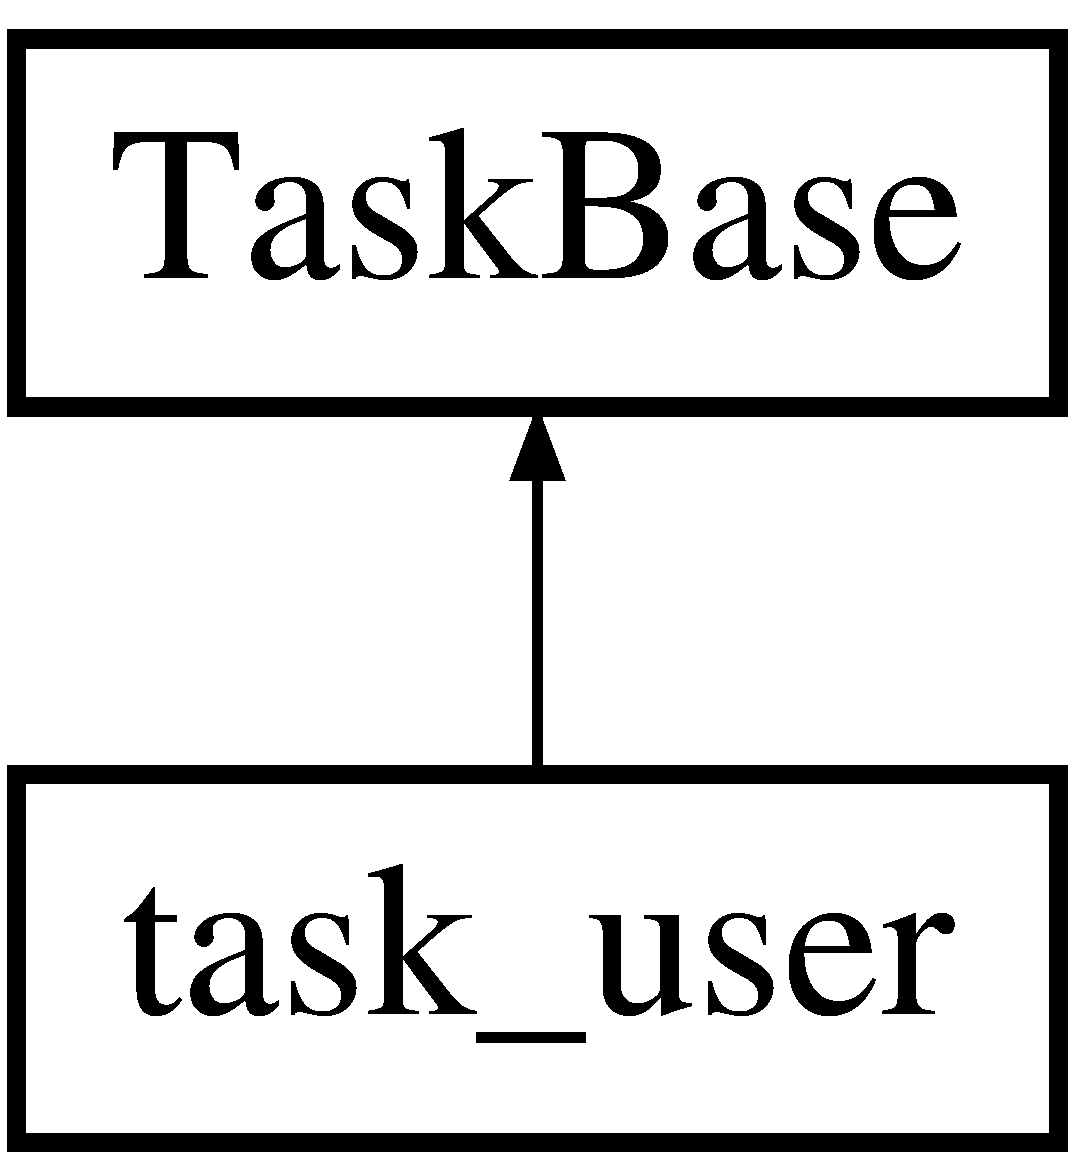
\includegraphics[height=2.000000cm]{classtask__user}
\end{center}
\end{figure}
\subsection*{Public Member Functions}
\begin{DoxyCompactItemize}
\item 
\hyperlink{classtask__user_a3aba77563b375bb14838800608da48bc}{task\-\_\-user} (const char $\ast$, unsigned port\-B\-A\-S\-E\-\_\-\-T\-Y\-P\-E, size\-\_\-t, emstream $\ast$)
\begin{DoxyCompactList}\small\item\em This constructor creates a user interface task object. \end{DoxyCompactList}\item 
void \hyperlink{classtask__user_adca6429d57be25e8d411414fc8ad75af}{run} (void)
\begin{DoxyCompactList}\small\item\em This method runs when the '\hyperlink{classtask__user}{task\-\_\-user}' is called. \end{DoxyCompactList}\end{DoxyCompactItemize}
\subsection*{Protected Member Functions}
\begin{DoxyCompactItemize}
\item 
void \hyperlink{classtask__user_a75475060f83bae1e44bcc8a5c34015c7}{print\-\_\-help\-\_\-message} (void)
\begin{DoxyCompactList}\small\item\em This method displays a simple help message telling the user what to do. \end{DoxyCompactList}\item 
void \hyperlink{classtask__user_a105bebbd9cb1031154c3dfc3662db4a0}{show\-\_\-status} (void)
\begin{DoxyCompactList}\small\item\em This method displays information about the status of the system. \end{DoxyCompactList}\item 
bool \hyperlink{classtask__user_aeebf78dc3a261ab26f137b9dedb4fae3}{has\-User\-Input} (void)
\begin{DoxyCompactList}\small\item\em Method returns true if the user has typed somthing into the terminal window. \end{DoxyCompactList}\item 
void \hyperlink{classtask__user_a6614555d84fb90fb2ae6c53a6e4ee7e6}{get\-Number\-Input} (void)
\begin{DoxyCompactList}\small\item\em Method extracts the number entered by the user and places it into private variable 'number\-\_\-entered'. \end{DoxyCompactList}\item 
void \hyperlink{classtask__user_a120498a0bdee78e47a42a1e6b8ee3ca9}{print\-Motor\-Menu} (void)
\begin{DoxyCompactList}\small\item\em Prints the opening menu when the user enters the 'Main Motor Module' in case1. \end{DoxyCompactList}\item 
void \hyperlink{classtask__user_ad7a5286a05c1782688037fd26c7e3d82}{print\-Main\-Menu} (void)
\begin{DoxyCompactList}\small\item\em Prints the Main Menu at the beginning of the program. \end{DoxyCompactList}\item 
void \hyperlink{classtask__user_a2866e8641ba983d7b819348a25774d47}{print\-Single\-Motor\-Options} (void)
\begin{DoxyCompactList}\small\item\em Prints the Single Motor Menu after the user has entered from the 'Main Motor Module'. \end{DoxyCompactList}\item 
void \hyperlink{classtask__user_affce6abe0cc4a021f490711a15234915}{print\-Dash\-Board} (void)
\begin{DoxyCompactList}\small\item\em Prints useful information about each motor like directive, power, and direction. \end{DoxyCompactList}\item 
void \hyperlink{classtask__user_ae247fa7d8dd68902ff4abf2c77b00fe2}{set\-Motor} (uint8\-\_\-t, int16\-\_\-t, uint8\-\_\-t)
\begin{DoxyCompactList}\small\item\em Method that takes the motor number, motor power, and directive and sets the correct motor to that directive at the apporpriate power level. \end{DoxyCompactList}\item 
void \hyperlink{classtask__user_a3ba42fcb41ae5292b75fe427ff26932c}{reset\-Menus} (void)
\begin{DoxyCompactList}\small\item\em This Method resets the 'run once' lock on each print menu method so that it can be run again. \end{DoxyCompactList}\item 
bool \hyperlink{classtask__user_a6178fb80b0e6fdebf254cc9aee6235a5}{is\-Valid\-Motor} (int16\-\_\-t)
\begin{DoxyCompactList}\small\item\em Method checks whether the motor number entered is valid and within range ($<$2) right now. \end{DoxyCompactList}\end{DoxyCompactItemize}
\subsection*{Protected Attributes}
\begin{DoxyCompactItemize}
\item 
\hypertarget{classtask__user_aeed69ce02fadbfb4a64758535e5c958b}{bool \hyperlink{classtask__user_aeed69ce02fadbfb4a64758535e5c958b}{is\-\_\-menu\-\_\-visible}}\label{classtask__user_aeed69ce02fadbfb4a64758535e5c958b}

\begin{DoxyCompactList}\small\item\em Holds true if there is a menu currently printed on the screen, false otherwise. \end{DoxyCompactList}\end{DoxyCompactItemize}


\subsection{Detailed Description}
This task will interact with the user and make the motors operate based on their input. 

Definition at line 79 of file task\-\_\-user.\-h.



\subsection{Constructor \& Destructor Documentation}
\hypertarget{classtask__user_a3aba77563b375bb14838800608da48bc}{\index{task\-\_\-user@{task\-\_\-user}!task\-\_\-user@{task\-\_\-user}}
\index{task\-\_\-user@{task\-\_\-user}!task_user@{task\-\_\-user}}
\subsubsection[{task\-\_\-user}]{\setlength{\rightskip}{0pt plus 5cm}task\-\_\-user\-::task\-\_\-user (
\begin{DoxyParamCaption}
\item[{const char $\ast$}]{a\-\_\-name, }
\item[{unsigned port\-B\-A\-S\-E\-\_\-\-T\-Y\-P\-E}]{a\-\_\-priority, }
\item[{size\-\_\-t}]{a\-\_\-stack\-\_\-size, }
\item[{emstream $\ast$}]{p\-\_\-ser\-\_\-dev}
\end{DoxyParamCaption}
)}}\label{classtask__user_a3aba77563b375bb14838800608da48bc}


This constructor creates a user interface task object. 

Constructor that creates a new task to interact with the user. All incoming paramters are initialized in the parent class construtor Task\-Base.

Added new initializations for private variables added in order to clean up the clutter in the main case statement in the '\hyperlink{classtask__user_adca6429d57be25e8d411414fc8ad75af}{run()}' method.


\begin{DoxyParams}[1]{Parameters}
\mbox{\tt in}  & {\em a\-\_\-name} & A character string which will be the name of this task \\
\hline
\mbox{\tt in}  & {\em a\-\_\-priority} & The priority at which this task will initially run (default\-: 0) \\
\hline
\mbox{\tt in}  & {\em a\-\_\-stack\-\_\-size} & The size of this task's stack in bytes (default\-: config\-M\-I\-N\-I\-M\-A\-L\-\_\-\-S\-T\-A\-C\-K\-\_\-\-S\-I\-Z\-E) \\
\hline
 & {\em p\-\_\-ser\-\_\-dev} & Pointer to a serial device (port, radio, S\-D card, etc. \\
\hline
\end{DoxyParams}


Definition at line 90 of file task\-\_\-user.\-cpp.



References F\-R\-E\-E\-W\-H\-E\-E\-L, and is\-\_\-menu\-\_\-visible.



\subsection{Member Function Documentation}
\hypertarget{classtask__user_a6614555d84fb90fb2ae6c53a6e4ee7e6}{\index{task\-\_\-user@{task\-\_\-user}!get\-Number\-Input@{get\-Number\-Input}}
\index{get\-Number\-Input@{get\-Number\-Input}!task_user@{task\-\_\-user}}
\subsubsection[{get\-Number\-Input}]{\setlength{\rightskip}{0pt plus 5cm}void task\-\_\-user\-::get\-Number\-Input (
\begin{DoxyParamCaption}
\item[{void}]{}
\end{DoxyParamCaption}
)\hspace{0.3cm}{\ttfamily [protected]}}}\label{classtask__user_a6614555d84fb90fb2ae6c53a6e4ee7e6}


Method extracts the number entered by the user and places it into private variable 'number\-\_\-entered'. 

Method gets the number being entered by the user.

This method uses a loop to constantly look for input until a return or escape symbol occurs. It then places the extracted negative or positive value in local class varible 'number\-\_\-entered'. 

Definition at line 668 of file task\-\_\-user.\-cpp.



References p\-\_\-print\-\_\-ser\-\_\-queue.



Referenced by run().

\hypertarget{classtask__user_aeebf78dc3a261ab26f137b9dedb4fae3}{\index{task\-\_\-user@{task\-\_\-user}!has\-User\-Input@{has\-User\-Input}}
\index{has\-User\-Input@{has\-User\-Input}!task_user@{task\-\_\-user}}
\subsubsection[{has\-User\-Input}]{\setlength{\rightskip}{0pt plus 5cm}bool task\-\_\-user\-::has\-User\-Input (
\begin{DoxyParamCaption}
\item[{void}]{}
\end{DoxyParamCaption}
)\hspace{0.3cm}{\ttfamily [protected]}}}\label{classtask__user_aeebf78dc3a261ab26f137b9dedb4fae3}


Method returns true if the user has typed somthing into the terminal window. 

Method checks if the user has made an input.

\begin{DoxyReturn}{Returns}
returns T\-R\-U\-E if the user has made an input and places that charater into the class variable 'char\-\_\-in'. Returns F\-A\-L\-S\-E otherwise. 
\end{DoxyReturn}


Definition at line 650 of file task\-\_\-user.\-cpp.



Referenced by run().

\hypertarget{classtask__user_a6178fb80b0e6fdebf254cc9aee6235a5}{\index{task\-\_\-user@{task\-\_\-user}!is\-Valid\-Motor@{is\-Valid\-Motor}}
\index{is\-Valid\-Motor@{is\-Valid\-Motor}!task_user@{task\-\_\-user}}
\subsubsection[{is\-Valid\-Motor}]{\setlength{\rightskip}{0pt plus 5cm}bool task\-\_\-user\-::is\-Valid\-Motor (
\begin{DoxyParamCaption}
\item[{int16\-\_\-t}]{motor\-\_\-number}
\end{DoxyParamCaption}
)\hspace{0.3cm}{\ttfamily [protected]}}}\label{classtask__user_a6178fb80b0e6fdebf254cc9aee6235a5}


Method checks whether the motor number entered is valid and within range ($<$2) right now. 

Method checks if the motor selected is a valid input.


\begin{DoxyParams}[1]{Parameters}
\mbox{\tt in}  & {\em motor\-\_\-number} & The number number entered by the user.\\
\hline
\end{DoxyParams}
\begin{DoxyReturn}{Returns}
returns T\-R\-U\-E if the motor value is valid, F\-A\-L\-S\-E otherwise 
\end{DoxyReturn}


Definition at line 803 of file task\-\_\-user.\-cpp.



Referenced by run().

\hypertarget{classtask__user_a75475060f83bae1e44bcc8a5c34015c7}{\index{task\-\_\-user@{task\-\_\-user}!print\-\_\-help\-\_\-message@{print\-\_\-help\-\_\-message}}
\index{print\-\_\-help\-\_\-message@{print\-\_\-help\-\_\-message}!task_user@{task\-\_\-user}}
\subsubsection[{print\-\_\-help\-\_\-message}]{\setlength{\rightskip}{0pt plus 5cm}void task\-\_\-user\-::print\-\_\-help\-\_\-message (
\begin{DoxyParamCaption}
\item[{void}]{}
\end{DoxyParamCaption}
)\hspace{0.3cm}{\ttfamily [protected]}}}\label{classtask__user_a75475060f83bae1e44bcc8a5c34015c7}


This method displays a simple help message telling the user what to do. 

This method contains the old main menu that has extra information and avaliable options. 

Definition at line 632 of file task\-\_\-user.\-cpp.



References P\-R\-O\-G\-R\-A\-M\-\_\-\-V\-E\-R\-S\-I\-O\-N.



Referenced by run().

\hypertarget{classtask__user_affce6abe0cc4a021f490711a15234915}{\index{task\-\_\-user@{task\-\_\-user}!print\-Dash\-Board@{print\-Dash\-Board}}
\index{print\-Dash\-Board@{print\-Dash\-Board}!task_user@{task\-\_\-user}}
\subsubsection[{print\-Dash\-Board}]{\setlength{\rightskip}{0pt plus 5cm}void task\-\_\-user\-::print\-Dash\-Board (
\begin{DoxyParamCaption}
\item[{void}]{}
\end{DoxyParamCaption}
)\hspace{0.3cm}{\ttfamily [protected]}}}\label{classtask__user_affce6abe0cc4a021f490711a15234915}


Prints useful information about each motor like directive, power, and direction. 

Method prints out useful information about both motors.

Only print the menu if the is\-\_\-menu\-\_\-visible flag is false. This is so that it doesn't inifinitely print as the user is trying to input a value or trying to read it. Furthermore, it prints out 'status', 'power', \& 'direction' 

Definition at line 523 of file task\-\_\-user.\-cpp.



References B\-R\-A\-K\-E, F\-R\-E\-E\-W\-H\-E\-E\-L, is\-\_\-menu\-\_\-visible, P\-O\-T\-E\-N\-T\-I\-O\-M\-E\-T\-E\-R, and S\-E\-T\-P\-O\-W\-E\-R.



Referenced by run().

\hypertarget{classtask__user_ad7a5286a05c1782688037fd26c7e3d82}{\index{task\-\_\-user@{task\-\_\-user}!print\-Main\-Menu@{print\-Main\-Menu}}
\index{print\-Main\-Menu@{print\-Main\-Menu}!task_user@{task\-\_\-user}}
\subsubsection[{print\-Main\-Menu}]{\setlength{\rightskip}{0pt plus 5cm}void task\-\_\-user\-::print\-Main\-Menu (
\begin{DoxyParamCaption}
\item[{void}]{}
\end{DoxyParamCaption}
)\hspace{0.3cm}{\ttfamily [protected]}}}\label{classtask__user_ad7a5286a05c1782688037fd26c7e3d82}


Prints the Main Menu at the beginning of the program. 

Method prints out the main menu, which is the first thing the user sees.

Menu is designed so that Control and testing modules are one part and all other operations like the ones included in the given version of this class are sectioned off accordingly. 

Definition at line 453 of file task\-\_\-user.\-cpp.



References is\-\_\-menu\-\_\-visible, and P\-R\-O\-G\-R\-A\-M\-\_\-\-V\-E\-R\-S\-I\-O\-N.



Referenced by run().

\hypertarget{classtask__user_a120498a0bdee78e47a42a1e6b8ee3ca9}{\index{task\-\_\-user@{task\-\_\-user}!print\-Motor\-Menu@{print\-Motor\-Menu}}
\index{print\-Motor\-Menu@{print\-Motor\-Menu}!task_user@{task\-\_\-user}}
\subsubsection[{print\-Motor\-Menu}]{\setlength{\rightskip}{0pt plus 5cm}void task\-\_\-user\-::print\-Motor\-Menu (
\begin{DoxyParamCaption}
\item[{void}]{}
\end{DoxyParamCaption}
)\hspace{0.3cm}{\ttfamily [protected]}}}\label{classtask__user_a120498a0bdee78e47a42a1e6b8ee3ca9}


Prints the opening menu when the user enters the 'Main Motor Module' in case1. 

Method prints out the 'Main Motor Module' menu.

Only print the menu if the is\-\_\-menu\-\_\-visible flag is false. This is so that it doesn't inifinitely print as the user is trying to input a value or trying to read it. 

Definition at line 478 of file task\-\_\-user.\-cpp.



References is\-\_\-menu\-\_\-visible.



Referenced by run().

\hypertarget{classtask__user_a2866e8641ba983d7b819348a25774d47}{\index{task\-\_\-user@{task\-\_\-user}!print\-Single\-Motor\-Options@{print\-Single\-Motor\-Options}}
\index{print\-Single\-Motor\-Options@{print\-Single\-Motor\-Options}!task_user@{task\-\_\-user}}
\subsubsection[{print\-Single\-Motor\-Options}]{\setlength{\rightskip}{0pt plus 5cm}void task\-\_\-user\-::print\-Single\-Motor\-Options (
\begin{DoxyParamCaption}
\item[{void}]{}
\end{DoxyParamCaption}
)\hspace{0.3cm}{\ttfamily [protected]}}}\label{classtask__user_a2866e8641ba983d7b819348a25774d47}


Prints the Single Motor Menu after the user has entered from the 'Main Motor Module'. 

Method prints out the 'Single Motor Control Module' menu.

Only print the menu if the is\-\_\-menu\-\_\-visible flag is false. This is so that it doesn't inifinitely print as the user is trying to input a value or trying to read it. 

Definition at line 501 of file task\-\_\-user.\-cpp.



References is\-\_\-menu\-\_\-visible.



Referenced by run().

\hypertarget{classtask__user_a3ba42fcb41ae5292b75fe427ff26932c}{\index{task\-\_\-user@{task\-\_\-user}!reset\-Menus@{reset\-Menus}}
\index{reset\-Menus@{reset\-Menus}!task_user@{task\-\_\-user}}
\subsubsection[{reset\-Menus}]{\setlength{\rightskip}{0pt plus 5cm}void task\-\_\-user\-::reset\-Menus (
\begin{DoxyParamCaption}
\item[{void}]{}
\end{DoxyParamCaption}
)\hspace{0.3cm}{\ttfamily [protected]}}}\label{classtask__user_a3ba42fcb41ae5292b75fe427ff26932c}


This Method resets the 'run once' lock on each print menu method so that it can be run again. 

Method resets the is\-\_\-menu\-\_\-visible flag so that another menu may be printed. 

Definition at line 816 of file task\-\_\-user.\-cpp.



References is\-\_\-menu\-\_\-visible.



Referenced by run().

\hypertarget{classtask__user_adca6429d57be25e8d411414fc8ad75af}{\index{task\-\_\-user@{task\-\_\-user}!run@{run}}
\index{run@{run}!task_user@{task\-\_\-user}}
\subsubsection[{run}]{\setlength{\rightskip}{0pt plus 5cm}void task\-\_\-user\-::run (
\begin{DoxyParamCaption}
\item[{void}]{}
\end{DoxyParamCaption}
)}}\label{classtask__user_adca6429d57be25e8d411414fc8ad75af}


This method runs when the '\hyperlink{classtask__user}{task\-\_\-user}' is called. 

This method is called by the R\-T\-O\-S once to run the task loop for ever and ever.

This method runs inifitely when the task is called so all logic is contained in here. A for(;;) loop runs until it gets to the end where it delays for 1 ms to allow other lower level priority tasks a chance to run. 

Definition at line 122 of file task\-\_\-user.\-cpp.



References B\-R\-A\-K\-E, F\-R\-E\-E\-W\-H\-E\-E\-L, get\-Number\-Input(), has\-User\-Input(), is\-Valid\-Motor(), motor\-\_\-power, motor\-\_\-select, P\-O\-T\-E\-N\-T\-I\-O\-M\-E\-T\-E\-R, print\-\_\-help\-\_\-message(), print\-Dash\-Board(), print\-Main\-Menu(), print\-Motor\-Menu(), print\-Single\-Motor\-Options(), reset\-Menus(), set\-Motor(), S\-E\-T\-P\-O\-W\-E\-R, and show\-\_\-status().

\hypertarget{classtask__user_ae247fa7d8dd68902ff4abf2c77b00fe2}{\index{task\-\_\-user@{task\-\_\-user}!set\-Motor@{set\-Motor}}
\index{set\-Motor@{set\-Motor}!task_user@{task\-\_\-user}}
\subsubsection[{set\-Motor}]{\setlength{\rightskip}{0pt plus 5cm}void task\-\_\-user\-::set\-Motor (
\begin{DoxyParamCaption}
\item[{uint8\-\_\-t}]{motor\-\_\-id, }
\item[{int16\-\_\-t}]{power, }
\item[{uint8\-\_\-t}]{direct}
\end{DoxyParamCaption}
)\hspace{0.3cm}{\ttfamily [protected]}}}\label{classtask__user_ae247fa7d8dd68902ff4abf2c77b00fe2}


Method that takes the motor number, motor power, and directive and sets the correct motor to that directive at the apporpriate power level. 

Method sets motor to the correct state as specified by user.

This method sets the global registers to the correct values so that '\hyperlink{classtask__motor}{task\-\_\-motor}' can affect the correct motor. Also sets appropriate local values to store the state of this motor so that when '\hyperlink{classtask__user_affce6abe0cc4a021f490711a15234915}{print\-Dash\-Board()}' is called it can print info on each motor because the global registers can only hold info for one motor at a time.


\begin{DoxyParams}[1]{Parameters}
\mbox{\tt in}  & {\em motor\-\_\-id} & The motor select identifier \\
\hline
\mbox{\tt in}  & {\em power} & The power setting specified by the user in the \hyperlink{classtask__user_adca6429d57be25e8d411414fc8ad75af}{run()} \\
\hline
\mbox{\tt in}  & {\em direct} & The directive, or what we want the motor to do \\
\hline
\end{DoxyParams}


Definition at line 776 of file task\-\_\-user.\-cpp.



References motor\-\_\-directive, motor\-\_\-power, and motor\-\_\-select.



Referenced by run().

\hypertarget{classtask__user_a105bebbd9cb1031154c3dfc3662db4a0}{\index{task\-\_\-user@{task\-\_\-user}!show\-\_\-status@{show\-\_\-status}}
\index{show\-\_\-status@{show\-\_\-status}!task_user@{task\-\_\-user}}
\subsubsection[{show\-\_\-status}]{\setlength{\rightskip}{0pt plus 5cm}void task\-\_\-user\-::show\-\_\-status (
\begin{DoxyParamCaption}
\item[{void}]{}
\end{DoxyParamCaption}
)\hspace{0.3cm}{\ttfamily [protected]}}}\label{classtask__user_a105bebbd9cb1031154c3dfc3662db4a0}


This method displays information about the status of the system. 

This method displays information about the status of the system, including the following\-: \begin{DoxyItemize}
\item The name and version of the program \item The name, status, priority, and free stack space of each task \item Processor cycles used by each task \item Amount of heap space free and setting of R\-T\-O\-S tick timer \end{DoxyItemize}


Definition at line 739 of file task\-\_\-user.\-cpp.



References P\-R\-O\-G\-R\-A\-M\-\_\-\-V\-E\-R\-S\-I\-O\-N.



Referenced by run().



The documentation for this class was generated from the following files\-:\begin{DoxyCompactItemize}
\item 
\hyperlink{task__user_8h}{task\-\_\-user.\-h}\item 
\hyperlink{task__user_8cpp}{task\-\_\-user.\-cpp}\end{DoxyCompactItemize}

\chapter{File Documentation}
\hypertarget{adc_8cpp}{
\section{adc.cpp File Reference}
\label{adc_8cpp}\index{adc.cpp@{adc.cpp}}
}
{\ttfamily \#include $<$stdlib.h$>$}\par
{\ttfamily \#include $<$avr/io.h$>$}\par
{\ttfamily \#include \char`\"{}rs232int.h\char`\"{}}\par
{\ttfamily \#include \char`\"{}adc.h\char`\"{}}\par
\subsection*{Functions}
\begin{DoxyCompactItemize}
\item 
emstream \& \hyperlink{adc_8cpp_afb33ca9fe94765ee57079e7feb03f975}{operator$<$$<$} (emstream \&serpt, \hyperlink{classadc}{adc} \&a2d)
\begin{DoxyCompactList}\small\item\em This overloaded operator \char`\"{}prints the A/D converter.\char`\"{}. \item\end{DoxyCompactList}\end{DoxyCompactItemize}


\subsection{Detailed Description}
This file contains a very simple A/D converter driver. This driver should be

Revisions: \begin{DoxyItemize}
\item 01-\/15-\/2008 JRR Original (somewhat useful) file \item 10-\/11-\/2012 JRR Less original, more useful file with FreeRTOS mutex added \item 10-\/12-\/2012 JRR There was a bug in the mutex code, and it has been fixed\end{DoxyItemize}
License: This file is copyright 2015 by JR Ridgely and released under the Lesser GNU Public License, version 2. It intended for educational use only, but its use is not limited thereto. 

Definition in file \hyperlink{adc_8cpp_source}{adc.cpp}.

\subsection{Function Documentation}
\hypertarget{adc_8cpp_afb33ca9fe94765ee57079e7feb03f975}{
\index{adc.cpp@{adc.cpp}!operator$<$$<$@{operator$<$$<$}}
\index{operator$<$$<$@{operator$<$$<$}!adc.cpp@{adc.cpp}}
\subsubsection[{operator$<$$<$}]{\setlength{\rightskip}{0pt plus 5cm}emstream\& operator$<$$<$ (emstream \& {\em serpt}, \/  {\bf adc} \& {\em a2d})}}
\label{adc_8cpp_afb33ca9fe94765ee57079e7feb03f975}


This overloaded operator \char`\"{}prints the A/D converter.\char`\"{}. The precise meaning of print is left to the user to interpret; it should be something useful. For example, one might print the values of the configuration registers or show current readings from all the A/D channels. 
\begin{DoxyParams}{Parameters}
\item[{\em serpt}]Reference to a serial port to which the printout will be printed \item[{\em a2d}]Reference to the A/D driver which is being printed \end{DoxyParams}
\begin{DoxyReturn}{Returns}
A reference to the same serial device on which we write information. This is used to string together things to write with {\ttfamily $<$$<$} operators 
\end{DoxyReturn}


Definition at line 133 of file adc.cpp.

References adc::read\_\-oversampled().
\hypertarget{adc_8h}{\section{adc.\-h File Reference}
\label{adc_8h}\index{adc.\-h@{adc.\-h}}
}
{\ttfamily \#include \char`\"{}emstream.\-h\char`\"{}}\\*
{\ttfamily \#include \char`\"{}Free\-R\-T\-O\-S.\-h\char`\"{}}\\*
{\ttfamily \#include \char`\"{}task.\-h\char`\"{}}\\*
{\ttfamily \#include \char`\"{}queue.\-h\char`\"{}}\\*
{\ttfamily \#include \char`\"{}semphr.\-h\char`\"{}}\\*
\subsection*{Classes}
\begin{DoxyCompactItemize}
\item 
class \hyperlink{classadc}{adc}
\begin{DoxyCompactList}\small\item\em This class {\bfseries will} run the A/\-D converter on an A\-V\-R processor. \end{DoxyCompactList}\end{DoxyCompactItemize}
\subsection*{Functions}
\begin{DoxyCompactItemize}
\item 
emstream \& \hyperlink{adc_8h_a6e6d1e227b216fe2a1fee9b0ea52180d}{operator$<$$<$} (emstream \&, \hyperlink{classadc}{adc} \&)
\begin{DoxyCompactList}\small\item\em This overloaded operator \char`\"{}prints the A/\-D converter.\char`\"{}. \end{DoxyCompactList}\end{DoxyCompactItemize}


\subsection{Detailed Description}
This file contains a very simple A/\-D converter driver. The driver is hopefully thread safe in Free\-R\-T\-O\-S due to the use of a mutex to prevent its use by multiple tasks at the same time. There is no protection from priority inversion, however, except for the priority elevation in the mutex.

Revisions\-: \begin{DoxyItemize}
\item 01-\/15-\/2008 J\-R\-R Original (somewhat useful) file \item 10-\/11-\/2012 J\-R\-R Less original, more useful file with Free\-R\-T\-O\-S mutex added \item 10-\/12-\/2012 J\-R\-R There was a bug in the mutex code, and it has been fixed\end{DoxyItemize}
License\-: This file is copyright 2012 by J\-R Ridgely and released under the Lesser G\-N\-U Public License, version 2. It intended for educational use only, but its use is not limited thereto. 

Definition in file \hyperlink{adc_8h_source}{adc.\-h}.



\subsection{Function Documentation}
\hypertarget{adc_8h_a6e6d1e227b216fe2a1fee9b0ea52180d}{\index{adc.\-h@{adc.\-h}!operator$<$$<$@{operator$<$$<$}}
\index{operator$<$$<$@{operator$<$$<$}!adc.h@{adc.\-h}}
\subsubsection[{operator$<$$<$}]{\setlength{\rightskip}{0pt plus 5cm}emstream\& operator$<$$<$ (
\begin{DoxyParamCaption}
\item[{emstream \&}]{serpt, }
\item[{{\bf adc} \&}]{a2d}
\end{DoxyParamCaption}
)}}\label{adc_8h_a6e6d1e227b216fe2a1fee9b0ea52180d}


This overloaded operator \char`\"{}prints the A/\-D converter.\char`\"{}. 

The precise meaning of print is left to the user to interpret; it should be something useful. For example, one might print the values of the configuration registers or show current readings from all the A/\-D channels. 
\begin{DoxyParams}{Parameters}
{\em serpt} & Reference to a serial port to which the printout will be printed \\
\hline
{\em a2d} & Reference to the A/\-D driver which is being printed \\
\hline
\end{DoxyParams}
\begin{DoxyReturn}{Returns}
A reference to the same serial device on which we write information. This is used to string together things to write with {\ttfamily $<$$<$} operators 
\end{DoxyReturn}


Definition at line 138 of file adc.\-cpp.


\hypertarget{main_8cpp}{\section{main.\-cpp File Reference}
\label{main_8cpp}\index{main.\-cpp@{main.\-cpp}}
}


This is the file for the '\hyperlink{main_8cpp_a840291bc02cba5474a4cb46a9b9566fe}{main()}' function. This function initialzies everything.  


{\ttfamily \#include $<$stdlib.\-h$>$}\\*
{\ttfamily \#include $<$avr/io.\-h$>$}\\*
{\ttfamily \#include $<$avr/wdt.\-h$>$}\\*
{\ttfamily \#include $<$string.\-h$>$}\\*
{\ttfamily \#include \char`\"{}Free\-R\-T\-O\-S.\-h\char`\"{}}\\*
{\ttfamily \#include \char`\"{}task.\-h\char`\"{}}\\*
{\ttfamily \#include \char`\"{}queue.\-h\char`\"{}}\\*
{\ttfamily \#include \char`\"{}croutine.\-h\char`\"{}}\\*
{\ttfamily \#include \char`\"{}rs232int.\-h\char`\"{}}\\*
{\ttfamily \#include \char`\"{}ansi\-\_\-terminal.\-h\char`\"{}}\\*
{\ttfamily \#include \char`\"{}time\-\_\-stamp.\-h\char`\"{}}\\*
{\ttfamily \#include \char`\"{}taskbase.\-h\char`\"{}}\\*
{\ttfamily \#include \char`\"{}textqueue.\-h\char`\"{}}\\*
{\ttfamily \#include \char`\"{}taskqueue.\-h\char`\"{}}\\*
{\ttfamily \#include \char`\"{}taskshare.\-h\char`\"{}}\\*
{\ttfamily \#include \char`\"{}shares.\-h\char`\"{}}\\*
{\ttfamily \#include \char`\"{}task\-\_\-brightness.\-h\char`\"{}}\\*
{\ttfamily \#include \char`\"{}task\-\_\-user.\-h\char`\"{}}\\*
{\ttfamily \#include \char`\"{}task\-\_\-motor.\-h\char`\"{}}\\*
{\ttfamily \#include \char`\"{}task\-\_\-encoder.\-h\char`\"{}}\\*
{\ttfamily \#include \char`\"{}hctl\-\_\-driver.\-h\char`\"{}}\\*
{\ttfamily \#include \char`\"{}imu\-\_\-driver.\-h\char`\"{}}\\*
{\ttfamily \#include \char`\"{}hctl.\-h\char`\"{}}\\*
{\ttfamily \#include \char`\"{}task\-\_\-pid.\-h\char`\"{}}\\*
\subsection*{Macros}
\begin{DoxyCompactItemize}
\item 
\hypertarget{main_8cpp_a523c5bde6173ed43b687f460b70648c1}{\#define \hyperlink{main_8cpp_a523c5bde6173ed43b687f460b70648c1}{N\-U\-L\-L\-\_\-\-M\-O\-T\-E\-R}~255}\label{main_8cpp_a523c5bde6173ed43b687f460b70648c1}

\begin{DoxyCompactList}\small\item\em Set the initital motor selector to something neutral. \end{DoxyCompactList}\end{DoxyCompactItemize}
\subsection*{Functions}
\begin{DoxyCompactItemize}
\item 
int \hyperlink{main_8cpp_a840291bc02cba5474a4cb46a9b9566fe}{main} (void)
\end{DoxyCompactItemize}
\subsection*{Variables}
\begin{DoxyCompactItemize}
\item 
Text\-Queue $\ast$ \hyperlink{main_8cpp_acd99bf5d187d4809af2f460a5415e904}{p\-\_\-print\-\_\-ser\-\_\-queue}
\item 
Task\-Share$<$ int16\-\_\-t $>$ $\ast$ \hyperlink{main_8cpp_a68e3aef51c9bd9903eca9b72f35fee2c}{motor\-\_\-setpoint}
\item 
Task\-Share$<$ int16\-\_\-t $>$ $\ast$ \hyperlink{main_8cpp_a94ed6a23dc3685572a19c9b35ad4d91b}{motor\-\_\-power}
\item 
Task\-Share$<$ uint8\-\_\-t $>$ $\ast$ \hyperlink{main_8cpp_a044692a403a6ad19401bd615cdefd5af}{motor\-\_\-directive}
\item 
\hypertarget{main_8cpp_a23620c74793eea7c070bd9799260bef4}{Task\-Share$<$ int32\-\_\-t $>$ $\ast$ \hyperlink{main_8cpp_a23620c74793eea7c070bd9799260bef4}{encoder\-\_\-count}}\label{main_8cpp_a23620c74793eea7c070bd9799260bef4}

\begin{DoxyCompactList}\small\item\em This variable holds the encoder count and is positive or negative relative to the rotation of the counts accumulated either Clock\-Wise(+), or Counter\-Clock\-Wise (-\/) \end{DoxyCompactList}\item 
\hypertarget{main_8cpp_ab8ab0b810225c2501e1952586bb99533}{Task\-Share$<$ int16\-\_\-t $>$ $\ast$ \hyperlink{main_8cpp_ab8ab0b810225c2501e1952586bb99533}{encoder\-\_\-ticks\-\_\-per\-\_\-task}}\label{main_8cpp_ab8ab0b810225c2501e1952586bb99533}

\begin{DoxyCompactList}\small\item\em This variable holds the ticks per seconds so that other tasks like task\-\_\-user may access it. \end{DoxyCompactList}\item 
\hypertarget{main_8cpp_ada2a13ebae63bc767f0c950ff1b8cb68}{Task\-Share$<$ uint32\-\_\-t $>$ $\ast$ \hyperlink{main_8cpp_ada2a13ebae63bc767f0c950ff1b8cb68}{data\-\_\-read}}\label{main_8cpp_ada2a13ebae63bc767f0c950ff1b8cb68}

\begin{DoxyCompactList}\small\item\em for I\-M\-U data read \end{DoxyCompactList}\item 
\hypertarget{main_8cpp_a0b55a56ebac94e7852175df8a4d45d27}{Task\-Share$<$ uint8\-\_\-t $>$ $\ast$ {\bfseries activate\-\_\-encoder}}\label{main_8cpp_a0b55a56ebac94e7852175df8a4d45d27}

\item 
\hypertarget{main_8cpp_a4d52cc8ed2fe6fdc27f652a6674829b8}{Task\-Share$<$ int16\-\_\-t $>$ $\ast$ {\bfseries steering\-\_\-power}}\label{main_8cpp_a4d52cc8ed2fe6fdc27f652a6674829b8}

\item 
\hypertarget{main_8cpp_af05c4a5de56d17ffcb642c090fab6a83}{Task\-Share$<$ int16\-\_\-t $>$ $\ast$ {\bfseries x\-\_\-joystick}}\label{main_8cpp_af05c4a5de56d17ffcb642c090fab6a83}

\item 
\hypertarget{main_8cpp_aab69cf68ba3a8e2382cce86f74bd5db4}{Task\-Share$<$ int16\-\_\-t $>$ $\ast$ {\bfseries y\-\_\-joystick}}\label{main_8cpp_aab69cf68ba3a8e2382cce86f74bd5db4}

\end{DoxyCompactItemize}


\subsection{Detailed Description}
This is the file for the '\hyperlink{main_8cpp_a840291bc02cba5474a4cb46a9b9566fe}{main()}' function. This function initialzies everything. Built on top of J\-R Ridgely's architecture, this modified \hyperlink{main_8cpp_a840291bc02cba5474a4cb46a9b9566fe}{main()} function initializes two motor\-\_\-driver$\ast$ objects, an A/\-D object. and various task\-Shares and tasks. Everything is initialized here and then propogated to other classes.

\begin{DoxyAuthor}{Author}
Eddie Ruano 

J\-R Ridgely
\end{DoxyAuthor}
Revisions\-: \begin{DoxyItemize}
\item 4/21/2016 created new motor tasks and gave them the correct pointer values. \item 4/19/2016 added new shared variables \item 09-\/30-\/2012 J\-R\-R Original file was a one-\/file demonstration with two tasks \item 10-\/05-\/2012 J\-R\-R Split into multiple files, one for each task plus a main one \item 10-\/30-\/2012 J\-R\-R A hopefully somewhat stable version with global queue pointers and the new operator used for most memory allocation \item 11-\/04-\/2012 J\-R\-R Free\-R\-T\-O\-S Swoop demo program changed to a sweet test suite \item 01-\/05-\/2012 J\-R\-R Program reconfigured as M\-E405 Lab 1 starting point \item 03-\/28-\/2014 J\-R\-R Pointers to shared variables and queues changed to references \item 01-\/04-\/2015 J\-R\-R Names of share \& queue classes changed allocated with new now License\-: This file is copyright 2012 by J\-R Ridgey and released under the Lesser G\-N\-U Public License, version 2. It intended for educational use only, but its use is not limited thereto. \end{DoxyItemize}


Definition in file \hyperlink{main_8cpp_source}{main.\-cpp}.



\subsection{Function Documentation}
\hypertarget{main_8cpp_a840291bc02cba5474a4cb46a9b9566fe}{\index{main.\-cpp@{main.\-cpp}!main@{main}}
\index{main@{main}!main.cpp@{main.\-cpp}}
\subsubsection[{main}]{\setlength{\rightskip}{0pt plus 5cm}int main (
\begin{DoxyParamCaption}
\item[{void}]{}
\end{DoxyParamCaption}
)}}\label{main_8cpp_a840291bc02cba5474a4cb46a9b9566fe}
The main function sets up the R\-T\-O\-S. Some test tasks are created. Then the scheduler is started up; the scheduler runs until power is turned off or there's a reset. \begin{DoxyReturn}{Returns}
This is a real-\/time microcontroller program which doesn't return. Ever. 
\end{DoxyReturn}


Definition at line 148 of file main.\-cpp.



References data\-\_\-read, encoder\-\_\-count, encoder\-\_\-ticks\-\_\-per\-\_\-task, motor\-\_\-directive, motor\-\_\-power, motor\-\_\-setpoint, and p\-\_\-print\-\_\-ser\-\_\-queue.



\subsection{Variable Documentation}
\hypertarget{main_8cpp_a044692a403a6ad19401bd615cdefd5af}{\index{main.\-cpp@{main.\-cpp}!motor\-\_\-directive@{motor\-\_\-directive}}
\index{motor\-\_\-directive@{motor\-\_\-directive}!main.cpp@{main.\-cpp}}
\subsubsection[{motor\-\_\-directive}]{\setlength{\rightskip}{0pt plus 5cm}Task\-Share$<$uint8\-\_\-t$>$$\ast$ motor\-\_\-directive}}\label{main_8cpp_a044692a403a6ad19401bd615cdefd5af}
This declares a taskshare which indicates that this variable is a shared variable. This variable will hold the command that the user wishes the motor to do. -\/1 Indicates C\-H\-A\-N\-G\-E\-\_\-\-D\-I\-R\-E\-C\-T\-I\-O\-N 0 Indicates S\-T\-O\-P W/ brake\-\_\-power 1 Indicates S\-E\-T P\-O\-W\-E\-R 2 Indicates F\-R\-E\-E\-W\-H\-E\-E\-L 

Definition at line 122 of file main.\-cpp.



Referenced by main().

\hypertarget{main_8cpp_a94ed6a23dc3685572a19c9b35ad4d91b}{\index{main.\-cpp@{main.\-cpp}!motor\-\_\-power@{motor\-\_\-power}}
\index{motor\-\_\-power@{motor\-\_\-power}!main.cpp@{main.\-cpp}}
\subsubsection[{motor\-\_\-power}]{\setlength{\rightskip}{0pt plus 5cm}Task\-Share$<$int16\-\_\-t$>$$\ast$ motor\-\_\-power}}\label{main_8cpp_a94ed6a23dc3685572a19c9b35ad4d91b}
This declares a taskshare which indicates that this variable is a shared variable. This variable will hold the duty cycle of a motor. 

Definition at line 114 of file main.\-cpp.



Referenced by main().

\hypertarget{main_8cpp_a68e3aef51c9bd9903eca9b72f35fee2c}{\index{main.\-cpp@{main.\-cpp}!motor\-\_\-setpoint@{motor\-\_\-setpoint}}
\index{motor\-\_\-setpoint@{motor\-\_\-setpoint}!main.cpp@{main.\-cpp}}
\subsubsection[{motor\-\_\-setpoint}]{\setlength{\rightskip}{0pt plus 5cm}Task\-Share$<$int16\-\_\-t$>$$\ast$ motor\-\_\-setpoint}}\label{main_8cpp_a68e3aef51c9bd9903eca9b72f35fee2c}
This declares a taskshare which indicates that this variable is a shared variable. This variable stores the setpoint for the P\-I\-D motor controller. 

Definition at line 110 of file main.\-cpp.



Referenced by main().

\hypertarget{main_8cpp_acd99bf5d187d4809af2f460a5415e904}{\index{main.\-cpp@{main.\-cpp}!p\-\_\-print\-\_\-ser\-\_\-queue@{p\-\_\-print\-\_\-ser\-\_\-queue}}
\index{p\-\_\-print\-\_\-ser\-\_\-queue@{p\-\_\-print\-\_\-ser\-\_\-queue}!main.cpp@{main.\-cpp}}
\subsubsection[{p\-\_\-print\-\_\-ser\-\_\-queue}]{\setlength{\rightskip}{0pt plus 5cm}Text\-Queue$\ast$ p\-\_\-print\-\_\-ser\-\_\-queue}}\label{main_8cpp_acd99bf5d187d4809af2f460a5415e904}
This is a print queue, descended from {\ttfamily emstream} so that things can be printed into the queue using the \char`\"{}$<$$<$\char`\"{} operator and they'll come out the other end as a stream of characters. It's used by tasks that send things to the user interface task to be printed. 

Definition at line 106 of file main.\-cpp.



Referenced by main().


\hypertarget{motor__driver_8cpp}{\section{motor\-\_\-driver.\-cpp File Reference}
\label{motor__driver_8cpp}\index{motor\-\_\-driver.\-cpp@{motor\-\_\-driver.\-cpp}}
}


This class is the motor driver class.  


{\ttfamily \#include $<$stdlib.\-h$>$}\\*
{\ttfamily \#include $<$avr/io.\-h$>$}\\*
{\ttfamily \#include \char`\"{}rs232int.\-h\char`\"{}}\\*
{\ttfamily \#include \char`\"{}motor\-\_\-driver.\-h\char`\"{}}\\*
\subsection*{Functions}
\begin{DoxyCompactItemize}
\item 
emstream \& \hyperlink{motor__driver_8cpp_ad657010257780226a5b845103f45f996}{operator$<$$<$} (emstream \&serpt, \hyperlink{classmotor__driver}{motor\-\_\-driver} \&motdrv)
\begin{DoxyCompactList}\small\item\em This overloaded operator prints information about a motor driver. \end{DoxyCompactList}\end{DoxyCompactItemize}


\subsection{Detailed Description}
This class is the motor driver class. This class creates an instance of a motor assuming caller gives all the correct and legal addresses and pin values, driver is able to map a motor to one of the two H bridge modules on the Custom M\-E 405 board.

\begin{DoxyAuthor}{Author}
Eddie Ruano
\end{DoxyAuthor}
Revisions\-: @ 4/23/2016 removed bitops.\-h library @ 4/16/2016 added bitops.\-h library for setting unsetting bits @ 4/12/2016 main structure created License\-: This file is copyright 2016 by Eddie Ruano and released under the Lesser G\-N\-U Public License, version 2. It intended for educational use only, but its use is not limited thereto. 

Definition in file \hyperlink{motor__driver_8cpp_source}{motor\-\_\-driver.\-cpp}.



\subsection{Function Documentation}
\hypertarget{motor__driver_8cpp_ad657010257780226a5b845103f45f996}{\index{motor\-\_\-driver.\-cpp@{motor\-\_\-driver.\-cpp}!operator$<$$<$@{operator$<$$<$}}
\index{operator$<$$<$@{operator$<$$<$}!motor_driver.cpp@{motor\-\_\-driver.\-cpp}}
\subsubsection[{operator$<$$<$}]{\setlength{\rightskip}{0pt plus 5cm}emstream\& operator$<$$<$ (
\begin{DoxyParamCaption}
\item[{emstream \&}]{serpt, }
\item[{{\bf motor\-\_\-driver} \&}]{motdrv}
\end{DoxyParamCaption}
)}}\label{motor__driver_8cpp_ad657010257780226a5b845103f45f996}


This overloaded operator prints information about a motor driver. 

It prints out appropriate information about the motor driver being delivered in the parameter.


\begin{DoxyParams}{Parameters}
{\em serpt} & A pointer to the serial port used. \\
\hline
{\em motdrv} & A pointer to a driver object\\
\hline
\end{DoxyParams}
\begin{DoxyReturn}{Returns}
A reference to the same serial device on which we write information. This is used to string together things to write with {\ttfamily $<$$<$} operators 
\end{DoxyReturn}


Definition at line 282 of file motor\-\_\-driver.\-cpp.



References motor\-\_\-driver\-::ocr\-\_\-\-P\-O\-R\-T.


\hypertarget{motor__driver_8h}{\section{motor\-\_\-driver.\-h File Reference}
\label{motor__driver_8h}\index{motor\-\_\-driver.\-h@{motor\-\_\-driver.\-h}}
}


This is the header file for the '\hyperlink{classmotor__driver}{motor\-\_\-driver}' class.  


{\ttfamily \#include \char`\"{}emstream.\-h\char`\"{}}\\*
{\ttfamily \#include \char`\"{}Free\-R\-T\-O\-S.\-h\char`\"{}}\\*
{\ttfamily \#include \char`\"{}task.\-h\char`\"{}}\\*
{\ttfamily \#include \char`\"{}queue.\-h\char`\"{}}\\*
{\ttfamily \#include \char`\"{}semphr.\-h\char`\"{}}\\*
\subsection*{Classes}
\begin{DoxyCompactItemize}
\item 
class \hyperlink{classmotor__driver}{motor\-\_\-driver}
\begin{DoxyCompactList}\small\item\em This class will run the D\-C motor. \end{DoxyCompactList}\end{DoxyCompactItemize}
\subsection*{Functions}
\begin{DoxyCompactItemize}
\item 
emstream \& \hyperlink{motor__driver_8h_a660b47b84ed9c985bfb681036ce37d7a}{operator$<$$<$} (emstream \&, \hyperlink{classmotor__driver}{motor\-\_\-driver} \&)
\begin{DoxyCompactList}\small\item\em This overloaded operator prints information about a motor driver. \end{DoxyCompactList}\end{DoxyCompactItemize}


\subsection{Detailed Description}
This is the header file for the '\hyperlink{classmotor__driver}{motor\-\_\-driver}' class. This is a task class that will control the operation of its own motor driver given to it as a pointer and initiated in the \hyperlink{main_8cpp_a840291bc02cba5474a4cb46a9b9566fe}{main()} function. it lays out the logic necessary to make commands from \hyperlink{classtask__user}{task\-\_\-user} to the motor driver happen.

\begin{DoxyAuthor}{Author}
Eddie Ruano
\end{DoxyAuthor}
Revisions\-: @ 4/23/2016 removed bitops.\-h library @ 4/16/2016 added bitops.\-h library for setting unsetting bits @ 4/12/2016 main structure created License\-: This file is copyright 2016 by Eddie Ruano and released under the Lesser G\-N\-U Public License, version 2. It intended for educational use only, but its use is not limited thereto. 

Definition in file \hyperlink{motor__driver_8h_source}{motor\-\_\-driver.\-h}.



\subsection{Function Documentation}
\hypertarget{motor__driver_8h_a660b47b84ed9c985bfb681036ce37d7a}{\index{motor\-\_\-driver.\-h@{motor\-\_\-driver.\-h}!operator$<$$<$@{operator$<$$<$}}
\index{operator$<$$<$@{operator$<$$<$}!motor_driver.h@{motor\-\_\-driver.\-h}}
\subsubsection[{operator$<$$<$}]{\setlength{\rightskip}{0pt plus 5cm}emstream\& operator$<$$<$ (
\begin{DoxyParamCaption}
\item[{emstream \&}]{serpt, }
\item[{{\bf motor\-\_\-driver} \&}]{motdrv}
\end{DoxyParamCaption}
)}}\label{motor__driver_8h_a660b47b84ed9c985bfb681036ce37d7a}


This overloaded operator prints information about a motor driver. 

It prints out appropriate information about the motor driver being delivered in the parameter.


\begin{DoxyParams}{Parameters}
{\em serpt} & A pointer to the serial port used. \\
\hline
{\em motdrv} & A pointer to a driver object\\
\hline
\end{DoxyParams}
\begin{DoxyReturn}{Returns}
A reference to the same serial device on which we write information. This is used to string together things to write with {\ttfamily $<$$<$} operators 
\end{DoxyReturn}


Definition at line 282 of file motor\-\_\-driver.\-cpp.



References motor\-\_\-driver\-::ocr\-\_\-\-P\-O\-R\-T.


\hypertarget{shares_8h}{\section{shares.\-h File Reference}
\label{shares_8h}\index{shares.\-h@{shares.\-h}}
}


This file contains extern declarations for queues and other inter-\/task data communication objects used in a M\-E405/507/\-Free\-R\-T\-O\-S project.  


\subsection*{Variables}
\begin{DoxyCompactItemize}
\item 
Text\-Queue $\ast$ \hyperlink{shares_8h_acd99bf5d187d4809af2f460a5415e904}{p\-\_\-print\-\_\-ser\-\_\-queue}
\item 
Task\-Share$<$ int16\-\_\-t $>$ $\ast$ \hyperlink{shares_8h_a94ed6a23dc3685572a19c9b35ad4d91b}{motor\-\_\-power}
\item 
Task\-Share$<$ uint8\-\_\-t $>$ $\ast$ \hyperlink{shares_8h_a044692a403a6ad19401bd615cdefd5af}{motor\-\_\-directive}
\item 
Task\-Share$<$ uint8\-\_\-t $>$ $\ast$ \hyperlink{shares_8h_a63b8526f83a43ed6aeb66f528aada7d6}{motor\-\_\-select}
\end{DoxyCompactItemize}


\subsection{Detailed Description}
This file contains extern declarations for queues and other inter-\/task data communication objects used in a M\-E405/507/\-Free\-R\-T\-O\-S project. This is a task class that will control the operation of its own motor driver given to it as a pointer and initiated in the \hyperlink{main_8cpp_a840291bc02cba5474a4cb46a9b9566fe}{main()} function. it lays out the logic necessary to make commands from \hyperlink{classtask__user}{task\-\_\-user} to the motor driver happen.

\begin{DoxyAuthor}{Author}
Eddie Ruano
\end{DoxyAuthor}
Revisions\-: \begin{DoxyItemize}
\item 4/20/2016 E\-R added more shares for the \hyperlink{classtask__motor}{task\-\_\-motor} operations \item 01-\/04-\/2014 J\-R\-R Re-\/reorganized, allocating shares with new now \item 09-\/30-\/2012 J\-R\-R Original file was a one-\/file demonstration with two tasks \item 10-\/05-\/2012 J\-R\-R Split into multiple files, one for each task plus a main one \item 10-\/29-\/2012 J\-R\-R Reorganized with global queue and shared data references License\-: This file is copyright 2016 by Eddie Ruano and released under the Lesser G\-N\-U Public License, version 2. It intended for educational use only, but its use is not limited thereto. \end{DoxyItemize}


Definition in file \hyperlink{shares_8h_source}{shares.\-h}.



\subsection{Variable Documentation}
\hypertarget{shares_8h_a044692a403a6ad19401bd615cdefd5af}{\index{shares.\-h@{shares.\-h}!motor\-\_\-directive@{motor\-\_\-directive}}
\index{motor\-\_\-directive@{motor\-\_\-directive}!shares.h@{shares.\-h}}
\subsubsection[{motor\-\_\-directive}]{\setlength{\rightskip}{0pt plus 5cm}Task\-Share$<$uint8\-\_\-t$>$$\ast$ motor\-\_\-directive}}\label{shares_8h_a044692a403a6ad19401bd615cdefd5af}
This declares a taskshare which indicates that this variable is a shared variable. This variable will hold the command that the user wishes the motor to do. 0 Indicates S\-E\-T P\-O\-W\-E\-R 1 Indicates B\-R\-A\-K\-E W/ brake\-\_\-power 2 Indicates F\-R\-E\-E\-W\-H\-E\-E\-L

This declares a taskshare which indicates that this variable is a shared variable. This variable will hold the command that the user wishes the motor to do. -\/1 Indicates C\-H\-A\-N\-G\-E\-\_\-\-D\-I\-R\-E\-C\-T\-I\-O\-N 0 Indicates S\-T\-O\-P W/ brake\-\_\-power 1 Indicates S\-E\-T P\-O\-W\-E\-R 2 Indicates F\-R\-E\-E\-W\-H\-E\-E\-L 

Definition at line 110 of file main.\-cpp.



Referenced by main(), task\-\_\-motor\-::run(), and task\-\_\-user\-::set\-Motor().

\hypertarget{shares_8h_a94ed6a23dc3685572a19c9b35ad4d91b}{\index{shares.\-h@{shares.\-h}!motor\-\_\-power@{motor\-\_\-power}}
\index{motor\-\_\-power@{motor\-\_\-power}!shares.h@{shares.\-h}}
\subsubsection[{motor\-\_\-power}]{\setlength{\rightskip}{0pt plus 5cm}Task\-Share$<$int16\-\_\-t$>$$\ast$ motor\-\_\-power}}\label{shares_8h_a94ed6a23dc3685572a19c9b35ad4d91b}
This declares a taskshare which indicates that this variable is a shared variable. This variable will hold the duty cycle of a motor. 

Definition at line 101 of file main.\-cpp.



Referenced by main(), task\-\_\-motor\-::run(), task\-\_\-user\-::run(), and task\-\_\-user\-::set\-Motor().

\hypertarget{shares_8h_a63b8526f83a43ed6aeb66f528aada7d6}{\index{shares.\-h@{shares.\-h}!motor\-\_\-select@{motor\-\_\-select}}
\index{motor\-\_\-select@{motor\-\_\-select}!shares.h@{shares.\-h}}
\subsubsection[{motor\-\_\-select}]{\setlength{\rightskip}{0pt plus 5cm}Task\-Share$<$uint8\-\_\-t$>$$\ast$ motor\-\_\-select}}\label{shares_8h_a63b8526f83a43ed6aeb66f528aada7d6}
This declares a taskshare which indicates that this variable is a shared variable. This variable will hold the select for each motor. 0 Indicates Motor 0 1 Indicates Motor 1 

Definition at line 117 of file main.\-cpp.



Referenced by main(), task\-\_\-motor\-::run(), task\-\_\-user\-::run(), and task\-\_\-user\-::set\-Motor().

\hypertarget{shares_8h_acd99bf5d187d4809af2f460a5415e904}{\index{shares.\-h@{shares.\-h}!p\-\_\-print\-\_\-ser\-\_\-queue@{p\-\_\-print\-\_\-ser\-\_\-queue}}
\index{p\-\_\-print\-\_\-ser\-\_\-queue@{p\-\_\-print\-\_\-ser\-\_\-queue}!shares.h@{shares.\-h}}
\subsubsection[{p\-\_\-print\-\_\-ser\-\_\-queue}]{\setlength{\rightskip}{0pt plus 5cm}Text\-Queue$\ast$ p\-\_\-print\-\_\-ser\-\_\-queue}}\label{shares_8h_acd99bf5d187d4809af2f460a5415e904}
This is a print queue, descended from {\ttfamily emstream} so that things can be printed into the queue using the \char`\"{}$<$$<$\char`\"{} operator and they'll come out the other end as a stream of characters. It's used by tasks that send things to the user interface task to be printed. 

Definition at line 96 of file main.\-cpp.



Referenced by task\-\_\-user\-::get\-Number\-Input(), and main().


\hypertarget{task__brightness_8cpp}{\section{task\-\_\-brightness.\-cpp File Reference}
\label{task__brightness_8cpp}\index{task\-\_\-brightness.\-cpp@{task\-\_\-brightness.\-cpp}}
}
{\ttfamily \#include \char`\"{}textqueue.\-h\char`\"{}}\\*
{\ttfamily \#include \char`\"{}task\-\_\-brightness.\-h\char`\"{}}\\*
{\ttfamily \#include \char`\"{}shares.\-h\char`\"{}}\\*


\subsection{Detailed Description}
This file contains the code for a task class which controls the brightness of an L\-E\-D using a voltage measured from the A/\-D as input. The fun part\-: the brightness that is being controlled can be on another A\-V\-R computer, with signals being sent and received via wireless transceivers.

Revisions\-: \begin{DoxyItemize}
\item 09-\/30-\/2012 J\-R\-R Original file was a one-\/file demonstration with two tasks \item 10-\/05-\/2012 J\-R\-R Split into multiple files, one for each task \item 10-\/25-\/2012 J\-R\-R Changed to a more fully C++ version with class task\-\_\-sender \item 10-\/27-\/2012 J\-R\-R Altered from data sending task into L\-E\-D blinking class \item 11-\/04-\/2012 J\-R\-R Altered again into the multi-\/task monstrosity \item 12-\/13-\/2012 J\-R\-R Yet again transmogrified; now it controls L\-E\-D brightness\end{DoxyItemize}
License\-: This file is copyright 2012 by J\-R Ridgely and released under the Lesser G\-N\-U Public License, version 2. It intended for educational use only, but its use is not limited thereto. 

Definition in file \hyperlink{task__brightness_8cpp_source}{task\-\_\-brightness.\-cpp}.


\hypertarget{task__brightness_8h}{
\section{task\_\-brightness.h File Reference}
\label{task__brightness_8h}\index{task\_\-brightness.h@{task\_\-brightness.h}}
}
{\ttfamily \#include $<$stdlib.h$>$}\par
{\ttfamily \#include $<$avr/io.h$>$}\par
{\ttfamily \#include \char`\"{}FreeRTOS.h\char`\"{}}\par
{\ttfamily \#include \char`\"{}task.h\char`\"{}}\par
{\ttfamily \#include \char`\"{}queue.h\char`\"{}}\par
{\ttfamily \#include \char`\"{}taskbase.h\char`\"{}}\par
{\ttfamily \#include \char`\"{}time\_\-stamp.h\char`\"{}}\par
{\ttfamily \#include \char`\"{}taskqueue.h\char`\"{}}\par
{\ttfamily \#include \char`\"{}taskshare.h\char`\"{}}\par
{\ttfamily \#include \char`\"{}rs232int.h\char`\"{}}\par
{\ttfamily \#include \char`\"{}adc.h\char`\"{}}\par
\subsection*{Classes}
\begin{DoxyCompactItemize}
\item 
class \hyperlink{classtask__brightness}{task\_\-brightness}
\begin{DoxyCompactList}\small\item\em This task controls the brightness of an LED using an analog input from the A/D converter. \item\end{DoxyCompactList}\end{DoxyCompactItemize}


\subsection{Detailed Description}
This file contains the header for a task class that controls the brightness of an LED using a voltage measured from the A/D as input. The fun part: the brightness that is being controlled can be on another AVR computer, with signals being sent and received via wireless transceivers.

Revisions: \begin{DoxyItemize}
\item 09-\/30-\/2012 JRR Original file was a one-\/file demonstration with two tasks \item 10-\/05-\/2012 JRR Split into multiple files, one for each task \item 10-\/25-\/2012 JRR Changed to a more fully C++ version with class task\_\-sender \item 10-\/27-\/2012 JRR Altered from data sending task into LED blinking class \item 11-\/04-\/2012 JRR Altered again into the multi-\/task monstrosity \item 12-\/13-\/2012 JRR Yet again transmogrified; now it controls LED brightness\end{DoxyItemize}
License: This file is copyright 2012 by JR Ridgely and released under the Lesser GNU Public License, version 2. It intended for educational use only, but its use is not limited thereto. 

Definition in file \hyperlink{task__brightness_8h_source}{task\_\-brightness.h}.
\hypertarget{task__motor_8cpp}{\section{task\-\_\-motor.\-cpp File Reference}
\label{task__motor_8cpp}\index{task\-\_\-motor.\-cpp@{task\-\_\-motor.\-cpp}}
}


This class is the task motor class that handles a single motor operation.  


{\ttfamily \#include \char`\"{}textqueue.\-h\char`\"{}}\\*
{\ttfamily \#include \char`\"{}task\-\_\-motor.\-h\char`\"{}}\\*
{\ttfamily \#include \char`\"{}shares.\-h\char`\"{}}\\*
\subsection*{Macros}
\begin{DoxyCompactItemize}
\item 
\hypertarget{task__motor_8cpp_af78f6af13b9c032bf9d48ef40aa7e683}{\#define \hyperlink{task__motor_8cpp_af78f6af13b9c032bf9d48ef40aa7e683}{B\-R\-A\-K\-E}~0}\label{task__motor_8cpp_af78f6af13b9c032bf9d48ef40aa7e683}

\begin{DoxyCompactList}\small\item\em Value for B\-R\-A\-K\-E directive. \end{DoxyCompactList}\item 
\hypertarget{task__motor_8cpp_add1d508d51340e49c96b0385ae4ad7d2}{\#define \hyperlink{task__motor_8cpp_add1d508d51340e49c96b0385ae4ad7d2}{S\-E\-T\-P\-O\-W\-E\-R}~1}\label{task__motor_8cpp_add1d508d51340e49c96b0385ae4ad7d2}

\begin{DoxyCompactList}\small\item\em Value for S\-E\-T\-P\-O\-W\-E\-R directive. \end{DoxyCompactList}\item 
\hypertarget{task__motor_8cpp_af9291ffc58d55b50465db4eb26e5b02d}{\#define \hyperlink{task__motor_8cpp_af9291ffc58d55b50465db4eb26e5b02d}{F\-R\-E\-E\-W\-H\-E\-E\-L}~2}\label{task__motor_8cpp_af9291ffc58d55b50465db4eb26e5b02d}

\begin{DoxyCompactList}\small\item\em Value for F\-R\-E\-E\-W\-H\-E\-E\-L directive. \end{DoxyCompactList}\item 
\hypertarget{task__motor_8cpp_a3e8e611e983546f51c69c43342fda6f2}{\#define \hyperlink{task__motor_8cpp_a3e8e611e983546f51c69c43342fda6f2}{P\-O\-T\-E\-N\-T\-I\-O\-M\-E\-T\-E\-R}~3}\label{task__motor_8cpp_a3e8e611e983546f51c69c43342fda6f2}

\begin{DoxyCompactList}\small\item\em Value for P\-O\-T\-E\-N\-T\-I\-O\-M\-E\-T\-E\-R directive. \end{DoxyCompactList}\end{DoxyCompactItemize}


\subsection{Detailed Description}
This class is the task motor class that handles a single motor operation. This is a task class that will control the operation of its own motor driver given to it as a pointer and initiated in the \hyperlink{main_8cpp_a840291bc02cba5474a4cb46a9b9566fe}{main()} function. it lays out the logic necessary to make commands from \hyperlink{classtask__user}{task\-\_\-user} to the motor driver happen.

\begin{DoxyAuthor}{Author}
Eddie Ruano
\end{DoxyAuthor}
Revisions\-: @ 4/20/2016 added main structure @ 4/22/2016 added pointers and correct logic License\-: This file is copyright 2016 by Eddie Ruano and released under the Lesser G\-N\-U Public License, version 2. It intended for educational use only, but its use is not limited thereto. 

Definition in file \hyperlink{task__motor_8cpp_source}{task\-\_\-motor.\-cpp}.


\hypertarget{task__motor_8h}{\section{task\-\_\-motor.\-h File Reference}
\label{task__motor_8h}\index{task\-\_\-motor.\-h@{task\-\_\-motor.\-h}}
}


This is the header file for the \hyperlink{classtask__motor}{task\-\_\-motor} class.  


{\ttfamily \#include $<$stdlib.\-h$>$}\\*
{\ttfamily \#include $<$avr/io.\-h$>$}\\*
{\ttfamily \#include \char`\"{}Free\-R\-T\-O\-S.\-h\char`\"{}}\\*
{\ttfamily \#include \char`\"{}task.\-h\char`\"{}}\\*
{\ttfamily \#include \char`\"{}queue.\-h\char`\"{}}\\*
{\ttfamily \#include \char`\"{}taskbase.\-h\char`\"{}}\\*
{\ttfamily \#include \char`\"{}time\-\_\-stamp.\-h\char`\"{}}\\*
{\ttfamily \#include \char`\"{}taskqueue.\-h\char`\"{}}\\*
{\ttfamily \#include \char`\"{}taskshare.\-h\char`\"{}}\\*
{\ttfamily \#include \char`\"{}rs232int.\-h\char`\"{}}\\*
{\ttfamily \#include \char`\"{}adc.\-h\char`\"{}}\\*
{\ttfamily \#include \char`\"{}motor\-\_\-driver.\-h\char`\"{}}\\*
\subsection*{Classes}
\begin{DoxyCompactItemize}
\item 
class \hyperlink{classtask__motor}{task\-\_\-motor}
\begin{DoxyCompactList}\small\item\em This class is the task motor class that handles a single motor operation. \end{DoxyCompactList}\end{DoxyCompactItemize}


\subsection{Detailed Description}
This is the header file for the \hyperlink{classtask__motor}{task\-\_\-motor} class. It lays out prototypes for the \hyperlink{classtask__motor}{task\-\_\-motor} constructor and the run class which is constantly called during operation. It also declared 3 local variables that hold a '\hyperlink{classmotor__driver}{motor\-\_\-driver}' pointer, a unsigned byte holding the task identifier (1 or 2) which is checked for at the beginning of the task logic and a pointer to an 'adc' A/\-D converter class.

\begin{DoxyAuthor}{Author}
Eddie Ruano
\end{DoxyAuthor}
Revisions\-: @ 4/20/2016 added main structure @ 4/22/2016 added pointers and correct logic License\-: This file is copyright 2016 by Eddie Ruano and released under the Lesser G\-N\-U Public License, version 2. It intended for educational use only, but its use is not limited thereto. 

Definition in file \hyperlink{task__motor_8h_source}{task\-\_\-motor.\-h}.


\hypertarget{task__user_8cpp}{\section{task\-\_\-user.\-cpp File Reference}
\label{task__user_8cpp}\index{task\-\_\-user.\-cpp@{task\-\_\-user.\-cpp}}
}


This is the file for the 'task\-\_\-user' class that is what any user will mainly interact with.  


{\ttfamily \#include $<$avr/io.\-h$>$}\\*
{\ttfamily \#include $<$avr/wdt.\-h$>$}\\*
{\ttfamily \#include \char`\"{}task\-\_\-user.\-h\char`\"{}}\\*
{\ttfamily \#include \char`\"{}ansi\-\_\-terminal.\-h\char`\"{}}\\*
{\ttfamily \#include \char`\"{}imu\-\_\-driver.\-h\char`\"{}}\\*
{\ttfamily \#include \char`\"{}task\-\_\-user\-\_\-library.\-h\char`\"{}}\\*
{\ttfamily \#include \char`\"{}adc.\-h\char`\"{}}\\*
\subsection*{Macros}
\begin{DoxyCompactItemize}
\item 
\hypertarget{task__user_8cpp_af78f6af13b9c032bf9d48ef40aa7e683}{\#define \hyperlink{task__user_8cpp_af78f6af13b9c032bf9d48ef40aa7e683}{B\-R\-A\-K\-E}~0}\label{task__user_8cpp_af78f6af13b9c032bf9d48ef40aa7e683}

\begin{DoxyCompactList}\small\item\em Value for B\-R\-A\-K\-E directive. \end{DoxyCompactList}\item 
\hypertarget{task__user_8cpp_add1d508d51340e49c96b0385ae4ad7d2}{\#define \hyperlink{task__user_8cpp_add1d508d51340e49c96b0385ae4ad7d2}{S\-E\-T\-P\-O\-W\-E\-R}~1}\label{task__user_8cpp_add1d508d51340e49c96b0385ae4ad7d2}

\begin{DoxyCompactList}\small\item\em Value for S\-E\-T\-P\-O\-W\-E\-R directive. \end{DoxyCompactList}\item 
\hypertarget{task__user_8cpp_af9291ffc58d55b50465db4eb26e5b02d}{\#define \hyperlink{task__user_8cpp_af9291ffc58d55b50465db4eb26e5b02d}{F\-R\-E\-E\-W\-H\-E\-E\-L}~2}\label{task__user_8cpp_af9291ffc58d55b50465db4eb26e5b02d}

\begin{DoxyCompactList}\small\item\em Value for F\-R\-E\-E\-W\-H\-E\-E\-L directive. \end{DoxyCompactList}\item 
\hypertarget{task__user_8cpp_a3e8e611e983546f51c69c43342fda6f2}{\#define \hyperlink{task__user_8cpp_a3e8e611e983546f51c69c43342fda6f2}{P\-O\-T\-E\-N\-T\-I\-O\-M\-E\-T\-E\-R}~3}\label{task__user_8cpp_a3e8e611e983546f51c69c43342fda6f2}

\begin{DoxyCompactList}\small\item\em Value for P\-O\-T\-E\-N\-T\-I\-O\-M\-E\-T\-E\-R directive. \end{DoxyCompactList}\end{DoxyCompactItemize}
\subsection*{Variables}
\begin{DoxyCompactItemize}
\item 
const Tick\-Type\-\_\-t \hyperlink{task__user_8cpp_a608f2ff6213a79bd1f25a29544aeaba5}{ticks\-\_\-to\-\_\-delay} = ((config\-T\-I\-C\-K\-\_\-\-R\-A\-T\-E\-\_\-\-H\-Z / 1000) $\ast$ 5)
\end{DoxyCompactItemize}


\subsection{Detailed Description}
This is the file for the 'task\-\_\-user' class that is what any user will mainly interact with. Built on top of J\-R Ridgely's architecture, this task uses case statements that infinitely loop in order to perform certain operations. In this version of this class (v1.\-1) the only module avaliable is the 'Main Motor Module' which allows the user to control both motors in on either H\-Bridge simultaneously.

\begin{DoxyAuthor}{Author}
Eddie Ruano 

J\-R Ridgely
\end{DoxyAuthor}
Revisions\-: \begin{DoxyItemize}
\item 4/26/2016 E\-R\-R added a new module for testing of the encoder task \item 4/23/2016 added a bunch of helper methods to make testing easier in the future \item 4/21/2016 overhauled entire case structure \item 09-\/30-\/2012 J\-R\-R Original file was a one-\/file demonstration with two tasks \item 10-\/05-\/2012 J\-R\-R Split into multiple files, one for each task \item 10-\/25-\/2012 J\-R\-R Changed to a more fully C++ version with class task\-\_\-user \item 11-\/04-\/2012 J\-R\-R Modified from the data acquisition example to the test suite \item 01-\/04-\/2014 J\-R\-R Changed base class names to Task\-Base, Task\-Share, etc. License\-: This file is copyright 2012 by J\-R Ridgey and released under the Lesser G\-N\-U Public License, version 2. It intended for educational use only, but its use is not limited thereto. \end{DoxyItemize}


Definition in file \hyperlink{task__user_8cpp_source}{task\-\_\-user.\-cpp}.



\subsection{Variable Documentation}
\hypertarget{task__user_8cpp_a608f2ff6213a79bd1f25a29544aeaba5}{\index{task\-\_\-user.\-cpp@{task\-\_\-user.\-cpp}!ticks\-\_\-to\-\_\-delay@{ticks\-\_\-to\-\_\-delay}}
\index{ticks\-\_\-to\-\_\-delay@{ticks\-\_\-to\-\_\-delay}!task_user.cpp@{task\-\_\-user.\-cpp}}
\subsubsection[{ticks\-\_\-to\-\_\-delay}]{\setlength{\rightskip}{0pt plus 5cm}const Tick\-Type\-\_\-t ticks\-\_\-to\-\_\-delay = ((config\-T\-I\-C\-K\-\_\-\-R\-A\-T\-E\-\_\-\-H\-Z / 1000) $\ast$ 5)}}\label{task__user_8cpp_a608f2ff6213a79bd1f25a29544aeaba5}
This constant sets how many R\-T\-O\-S ticks the task delays if the user's not talking The duration is calculated to be about 5 ms. 

Definition at line 81 of file task\-\_\-user.\-cpp.


\hypertarget{task__user_8h}{\section{task\-\_\-user.\-h File Reference}
\label{task__user_8h}\index{task\-\_\-user.\-h@{task\-\_\-user.\-h}}
}


This is the header file for the '\hyperlink{classtask__user}{task\-\_\-user}' class.  


{\ttfamily \#include $<$stdlib.\-h$>$}\\*
{\ttfamily \#include \char`\"{}Free\-R\-T\-O\-S.\-h\char`\"{}}\\*
{\ttfamily \#include \char`\"{}task.\-h\char`\"{}}\\*
{\ttfamily \#include \char`\"{}queue.\-h\char`\"{}}\\*
{\ttfamily \#include \char`\"{}rs232int.\-h\char`\"{}}\\*
{\ttfamily \#include \char`\"{}adc.\-h\char`\"{}}\\*
{\ttfamily \#include \char`\"{}motor\-\_\-driver.\-h\char`\"{}}\\*
{\ttfamily \#include \char`\"{}time\-\_\-stamp.\-h\char`\"{}}\\*
{\ttfamily \#include \char`\"{}taskbase.\-h\char`\"{}}\\*
{\ttfamily \#include \char`\"{}taskqueue.\-h\char`\"{}}\\*
{\ttfamily \#include \char`\"{}textqueue.\-h\char`\"{}}\\*
{\ttfamily \#include \char`\"{}taskshare.\-h\char`\"{}}\\*
{\ttfamily \#include \char`\"{}shares.\-h\char`\"{}}\\*
\subsection*{Classes}
\begin{DoxyCompactItemize}
\item 
class \hyperlink{classtask__user}{task\-\_\-user}
\begin{DoxyCompactList}\small\item\em This task will interact with the user and make the motors operate based on their input. \end{DoxyCompactList}\end{DoxyCompactItemize}
\subsection*{Macros}
\begin{DoxyCompactItemize}
\item 
\#define \hyperlink{task__user_8h_a2f10abd650e471fae2d7e8c63d41206a}{P\-R\-O\-G\-R\-A\-M\-\_\-\-V\-E\-R\-S\-I\-O\-N}~P\-M\-S (\char`\"{}M\-E405 Lab 3 Encoder Driver Integration\char`\"{})
\end{DoxyCompactItemize}


\subsection{Detailed Description}
This is the header file for the '\hyperlink{classtask__user}{task\-\_\-user}' class. Built on top of J\-R Ridgely's architecture, this header lays out all the protoypes and local variables used in the '\hyperlink{classtask__user}{task\-\_\-user}' class.

\begin{DoxyAuthor}{Author}
Eddie Ruano 

J\-R Ridgely
\end{DoxyAuthor}
Revisions\-: \begin{DoxyItemize}
\item 4/20/2016 added main structure \item 4/22/2016 added pointers and correct logic \item 09-\/30-\/2012 J\-R\-R Original file was a one-\/file demonstration with two tasks \item 10-\/05-\/2012 J\-R\-R Split into multiple files, one for each task \item 10-\/25-\/2012 J\-R\-R Changed to a more fully C++ version with class \hyperlink{classtask__user}{task\-\_\-user} \item 11-\/04-\/2012 J\-R\-R Modified from the data acquisition example to the test suite \item 01-\/04-\/2014 J\-R\-R Changed base class names to Task\-Base, Task\-Share, etc. License\-: This file is copyright 2016 by Eddie Ruano and released under the Lesser G\-N\-U Public License, version 2. It intended for educational use only, but its use is not limited thereto. \end{DoxyItemize}


Definition in file \hyperlink{task__user_8h_source}{task\-\_\-user.\-h}.



\subsection{Macro Definition Documentation}
\hypertarget{task__user_8h_a2f10abd650e471fae2d7e8c63d41206a}{\index{task\-\_\-user.\-h@{task\-\_\-user.\-h}!P\-R\-O\-G\-R\-A\-M\-\_\-\-V\-E\-R\-S\-I\-O\-N@{P\-R\-O\-G\-R\-A\-M\-\_\-\-V\-E\-R\-S\-I\-O\-N}}
\index{P\-R\-O\-G\-R\-A\-M\-\_\-\-V\-E\-R\-S\-I\-O\-N@{P\-R\-O\-G\-R\-A\-M\-\_\-\-V\-E\-R\-S\-I\-O\-N}!task_user.h@{task\-\_\-user.\-h}}
\subsubsection[{P\-R\-O\-G\-R\-A\-M\-\_\-\-V\-E\-R\-S\-I\-O\-N}]{\setlength{\rightskip}{0pt plus 5cm}\#define P\-R\-O\-G\-R\-A\-M\-\_\-\-V\-E\-R\-S\-I\-O\-N~P\-M\-S (\char`\"{}M\-E405 Lab 3 Encoder Driver Integration\char`\"{})}}\label{task__user_8h_a2f10abd650e471fae2d7e8c63d41206a}
This macro defines a string that identifies the name and version of this program. 

Definition at line 72 of file task\-\_\-user.\-h.



Referenced by task\-\_\-user\-::print\-\_\-help\-\_\-message(), task\-\_\-user\-::print\-Main\-Menu(), and task\-\_\-user\-::show\-\_\-status().


%--- End generated contents ---

% Index
\newpage
\phantomsection
\addcontentsline{toc}{chapter}{Index}
\printindex

\end{document}
